% Options for packages loaded elsewhere
\PassOptionsToPackage{unicode}{hyperref}
\PassOptionsToPackage{hyphens}{url}
\documentclass[
]{article}
\usepackage{xcolor}
\usepackage[margin=1in]{geometry}
\usepackage{amsmath,amssymb}
\setcounter{secnumdepth}{5}
\usepackage{iftex}
\ifPDFTeX
  \usepackage[T1]{fontenc}
  \usepackage[utf8]{inputenc}
  \usepackage{textcomp} % provide euro and other symbols
\else % if luatex or xetex
  \usepackage{unicode-math} % this also loads fontspec
  \defaultfontfeatures{Scale=MatchLowercase}
  \defaultfontfeatures[\rmfamily]{Ligatures=TeX,Scale=1}
\fi
\usepackage{lmodern}
\ifPDFTeX\else
  % xetex/luatex font selection
\fi
% Use upquote if available, for straight quotes in verbatim environments
\IfFileExists{upquote.sty}{\usepackage{upquote}}{}
\IfFileExists{microtype.sty}{% use microtype if available
  \usepackage[]{microtype}
  \UseMicrotypeSet[protrusion]{basicmath} % disable protrusion for tt fonts
}{}
\makeatletter
\@ifundefined{KOMAClassName}{% if non-KOMA class
  \IfFileExists{parskip.sty}{%
    \usepackage{parskip}
  }{% else
    \setlength{\parindent}{0pt}
    \setlength{\parskip}{6pt plus 2pt minus 1pt}}
}{% if KOMA class
  \KOMAoptions{parskip=half}}
\makeatother
\usepackage{color}
\usepackage{fancyvrb}
\newcommand{\VerbBar}{|}
\newcommand{\VERB}{\Verb[commandchars=\\\{\}]}
\DefineVerbatimEnvironment{Highlighting}{Verbatim}{commandchars=\\\{\}}
% Add ',fontsize=\small' for more characters per line
\usepackage{framed}
\definecolor{shadecolor}{RGB}{248,248,248}
\newenvironment{Shaded}{\begin{snugshade}}{\end{snugshade}}
\newcommand{\AlertTok}[1]{\textcolor[rgb]{0.94,0.16,0.16}{#1}}
\newcommand{\AnnotationTok}[1]{\textcolor[rgb]{0.56,0.35,0.01}{\textbf{\textit{#1}}}}
\newcommand{\AttributeTok}[1]{\textcolor[rgb]{0.13,0.29,0.53}{#1}}
\newcommand{\BaseNTok}[1]{\textcolor[rgb]{0.00,0.00,0.81}{#1}}
\newcommand{\BuiltInTok}[1]{#1}
\newcommand{\CharTok}[1]{\textcolor[rgb]{0.31,0.60,0.02}{#1}}
\newcommand{\CommentTok}[1]{\textcolor[rgb]{0.56,0.35,0.01}{\textit{#1}}}
\newcommand{\CommentVarTok}[1]{\textcolor[rgb]{0.56,0.35,0.01}{\textbf{\textit{#1}}}}
\newcommand{\ConstantTok}[1]{\textcolor[rgb]{0.56,0.35,0.01}{#1}}
\newcommand{\ControlFlowTok}[1]{\textcolor[rgb]{0.13,0.29,0.53}{\textbf{#1}}}
\newcommand{\DataTypeTok}[1]{\textcolor[rgb]{0.13,0.29,0.53}{#1}}
\newcommand{\DecValTok}[1]{\textcolor[rgb]{0.00,0.00,0.81}{#1}}
\newcommand{\DocumentationTok}[1]{\textcolor[rgb]{0.56,0.35,0.01}{\textbf{\textit{#1}}}}
\newcommand{\ErrorTok}[1]{\textcolor[rgb]{0.64,0.00,0.00}{\textbf{#1}}}
\newcommand{\ExtensionTok}[1]{#1}
\newcommand{\FloatTok}[1]{\textcolor[rgb]{0.00,0.00,0.81}{#1}}
\newcommand{\FunctionTok}[1]{\textcolor[rgb]{0.13,0.29,0.53}{\textbf{#1}}}
\newcommand{\ImportTok}[1]{#1}
\newcommand{\InformationTok}[1]{\textcolor[rgb]{0.56,0.35,0.01}{\textbf{\textit{#1}}}}
\newcommand{\KeywordTok}[1]{\textcolor[rgb]{0.13,0.29,0.53}{\textbf{#1}}}
\newcommand{\NormalTok}[1]{#1}
\newcommand{\OperatorTok}[1]{\textcolor[rgb]{0.81,0.36,0.00}{\textbf{#1}}}
\newcommand{\OtherTok}[1]{\textcolor[rgb]{0.56,0.35,0.01}{#1}}
\newcommand{\PreprocessorTok}[1]{\textcolor[rgb]{0.56,0.35,0.01}{\textit{#1}}}
\newcommand{\RegionMarkerTok}[1]{#1}
\newcommand{\SpecialCharTok}[1]{\textcolor[rgb]{0.81,0.36,0.00}{\textbf{#1}}}
\newcommand{\SpecialStringTok}[1]{\textcolor[rgb]{0.31,0.60,0.02}{#1}}
\newcommand{\StringTok}[1]{\textcolor[rgb]{0.31,0.60,0.02}{#1}}
\newcommand{\VariableTok}[1]{\textcolor[rgb]{0.00,0.00,0.00}{#1}}
\newcommand{\VerbatimStringTok}[1]{\textcolor[rgb]{0.31,0.60,0.02}{#1}}
\newcommand{\WarningTok}[1]{\textcolor[rgb]{0.56,0.35,0.01}{\textbf{\textit{#1}}}}
\usepackage{graphicx}
\makeatletter
\newsavebox\pandoc@box
\newcommand*\pandocbounded[1]{% scales image to fit in text height/width
  \sbox\pandoc@box{#1}%
  \Gscale@div\@tempa{\textheight}{\dimexpr\ht\pandoc@box+\dp\pandoc@box\relax}%
  \Gscale@div\@tempb{\linewidth}{\wd\pandoc@box}%
  \ifdim\@tempb\p@<\@tempa\p@\let\@tempa\@tempb\fi% select the smaller of both
  \ifdim\@tempa\p@<\p@\scalebox{\@tempa}{\usebox\pandoc@box}%
  \else\usebox{\pandoc@box}%
  \fi%
}
% Set default figure placement to htbp
\def\fps@figure{htbp}
\makeatother
\setlength{\emergencystretch}{3em} % prevent overfull lines
\providecommand{\tightlist}{%
  \setlength{\itemsep}{0pt}\setlength{\parskip}{0pt}}
\usepackage[]{natbib}
\bibliographystyle{plainnat}
\usepackage{bookmark}
\IfFileExists{xurl.sty}{\usepackage{xurl}}{} % add URL line breaks if available
\urlstyle{same}
\hypersetup{
  pdftitle={Lab 01 - Hello R!},
  hidelinks,
  pdfcreator={LaTeX via pandoc}}

\title{Lab 01 - Hello R!}
\author{}
\date{\vspace{-2.5em}}

\begin{document}
\maketitle

{
\setcounter{tocdepth}{2}
\tableofcontents
}
\begin{Shaded}
\begin{Highlighting}[]
\NormalTok{R is the name of the programming language itself and RStudio is a convenient interface.}
\end{Highlighting}
\end{Shaded}

The main goal of this lab is to introduce you to R and RStudio, which we
will be using throughout the course both to learn the statistical
concepts discussed in the course and to analyze real data and come to
informed conclusions.

\begin{Shaded}
\begin{Highlighting}[]
\NormalTok{git is a version control system (like "Track Changes" features from Microsoft Word on steroids) and GitHub is the home for your Git{-}based projects on the internet (like DropBox but much, much better).}
\end{Highlighting}
\end{Shaded}

An additional goal is to introduce you to Git and GitHub, which is the
collaboration and version control system that we will be using
throughout the course.

As the labs progress, you are encouraged to explore beyond what the labs
dictate; a willingness to experiment will make you a much better
programmer. Before we get to that stage, however, you need to build some
basic fluency in R. Today we begin with the fundamental building blocks
of R and RStudio: the interface, reading in data, and basic commands.

And to make versioning simpler, this is a solo lab. Additionally, we
want to make sure everyone gets a significant amount of time at the
steering wheel. In future labs you'll learn about collaborating on
GitHub and produce a single lab report for your team.

\section{Connecting GitHub and RStudio
Cloud}\label{connecting-github-and-rstudio-cloud}

You should have already received an invitation to join the GitHub
organization for this course. You need to accept the invitation before
moving on to the next step.

To connect your RStudio and GitHub accounts by following the steps
below:

\begin{itemize}
\tightlist
\item
  Click on your name on the top right corner to open the right menu.
\item
  Then, click on Authentication.
\end{itemize}

\pandocbounded{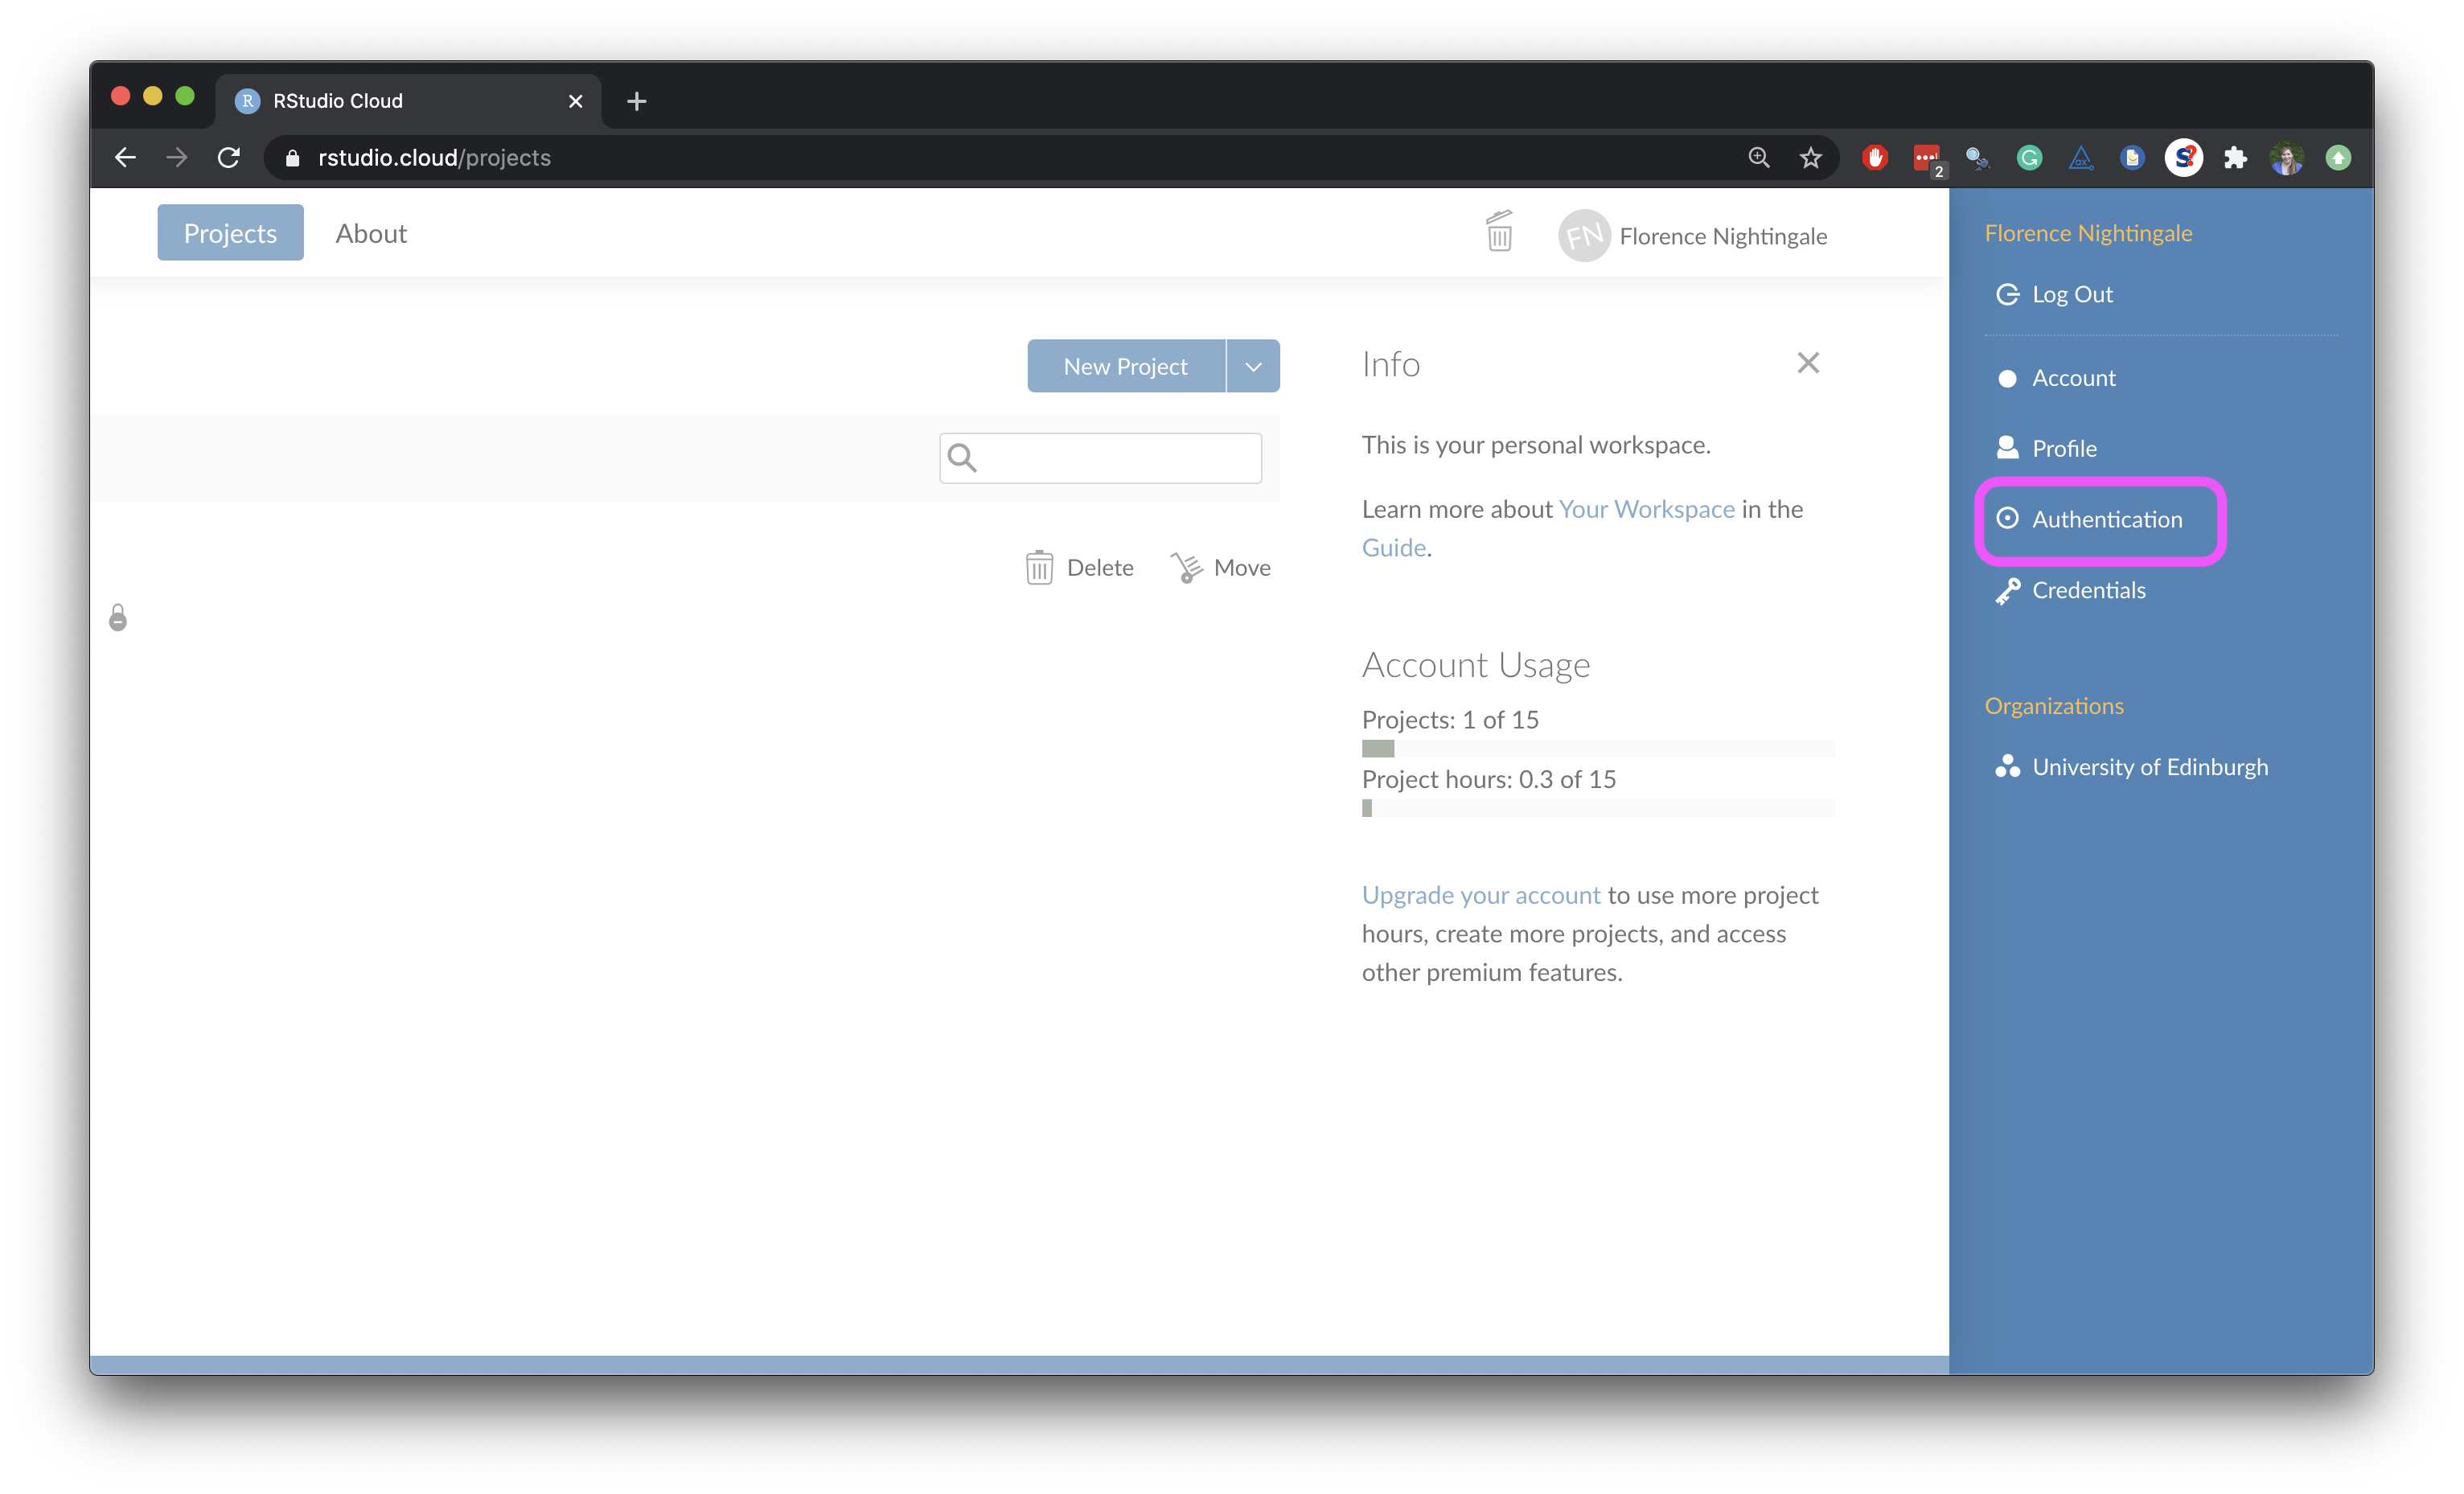
\includegraphics[keepaspectratio]{img/github-auth-1.png}}

\begin{itemize}
\tightlist
\item
  In the Authentication window, check the box for \emph{Enabled}.
\end{itemize}

\pandocbounded{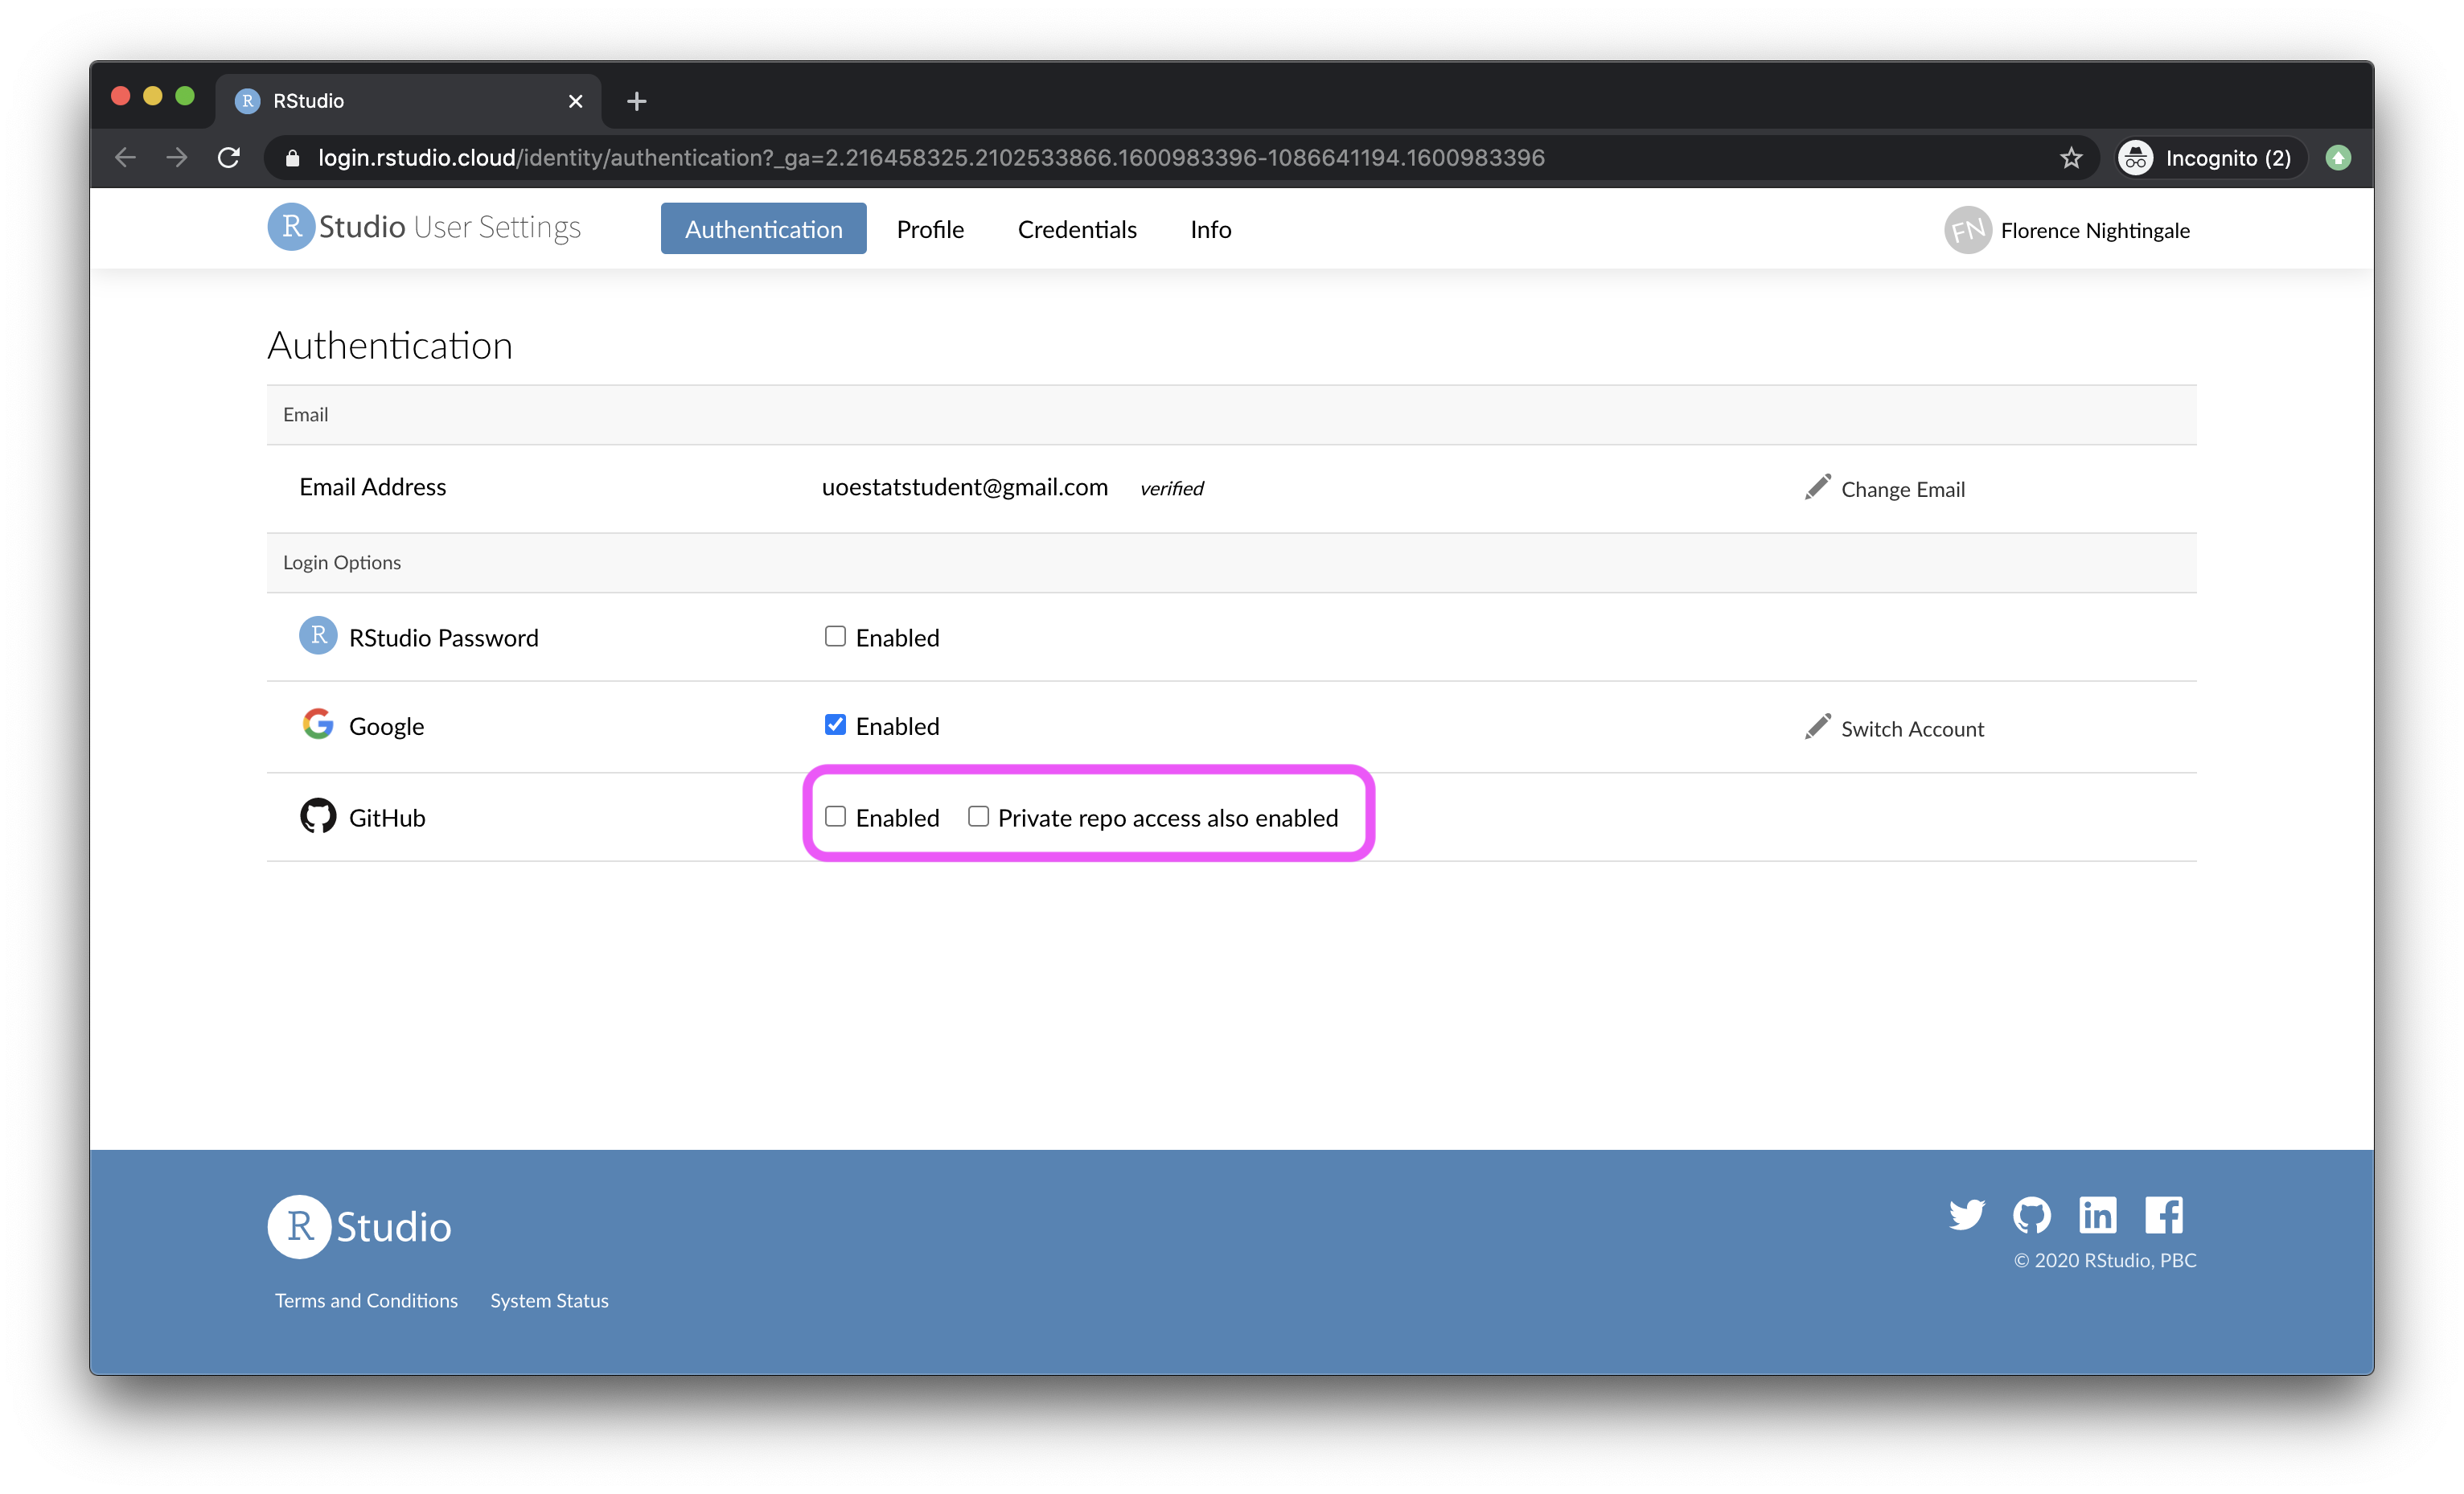
\includegraphics[keepaspectratio]{img/github-auth-2.png}}

\begin{itemize}
\tightlist
\item
  In the next window, click on the green box that says ``Authorize
  rstudio''.
\end{itemize}

\pandocbounded{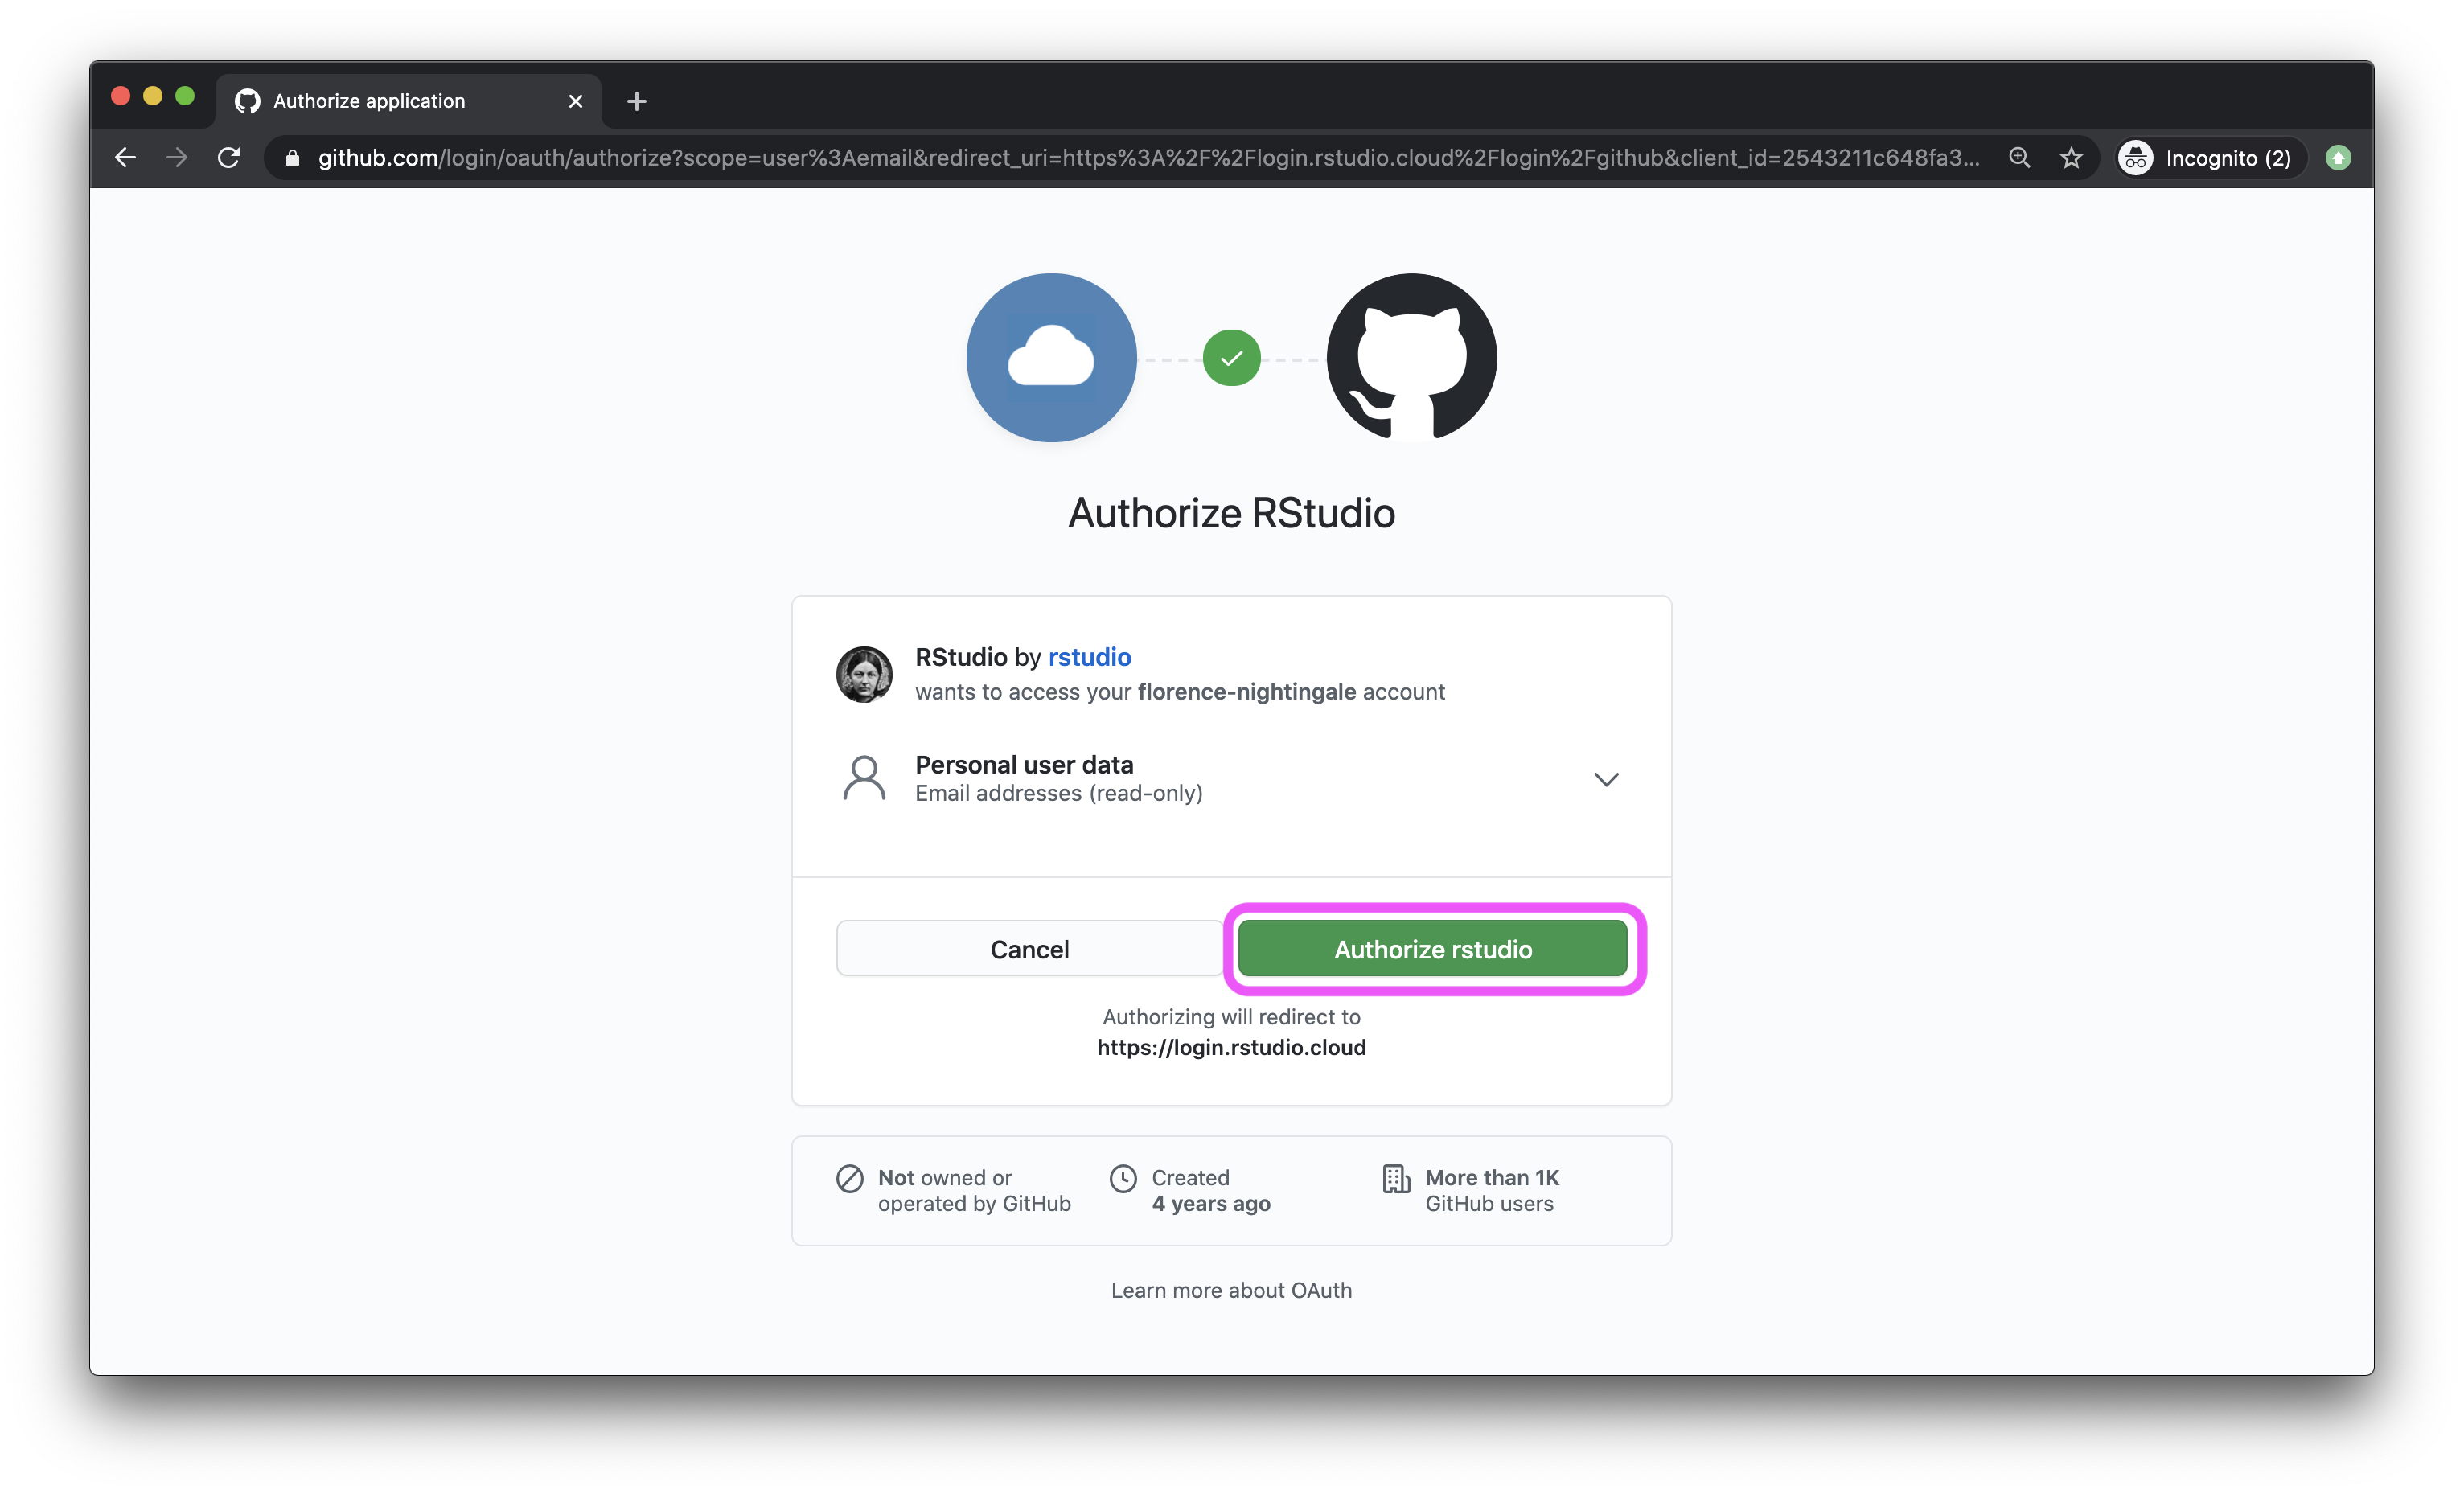
\includegraphics[keepaspectratio]{img/github-auth-3.png}}

\begin{itemize}
\tightlist
\item
  Back in the Authentication window, check the box for \emph{Private
  repo access also enabled}, and once again, on the green box that says
  ``Authorize rstudio'' in the next window. At this point you should
  also make sure that the course organization shows up for you under
  \emph{Organization access}. If it does not, this means you have not
  yet accepted the GitHub invitation to join the course, and you should
  go back and do that.
\end{itemize}

\pandocbounded{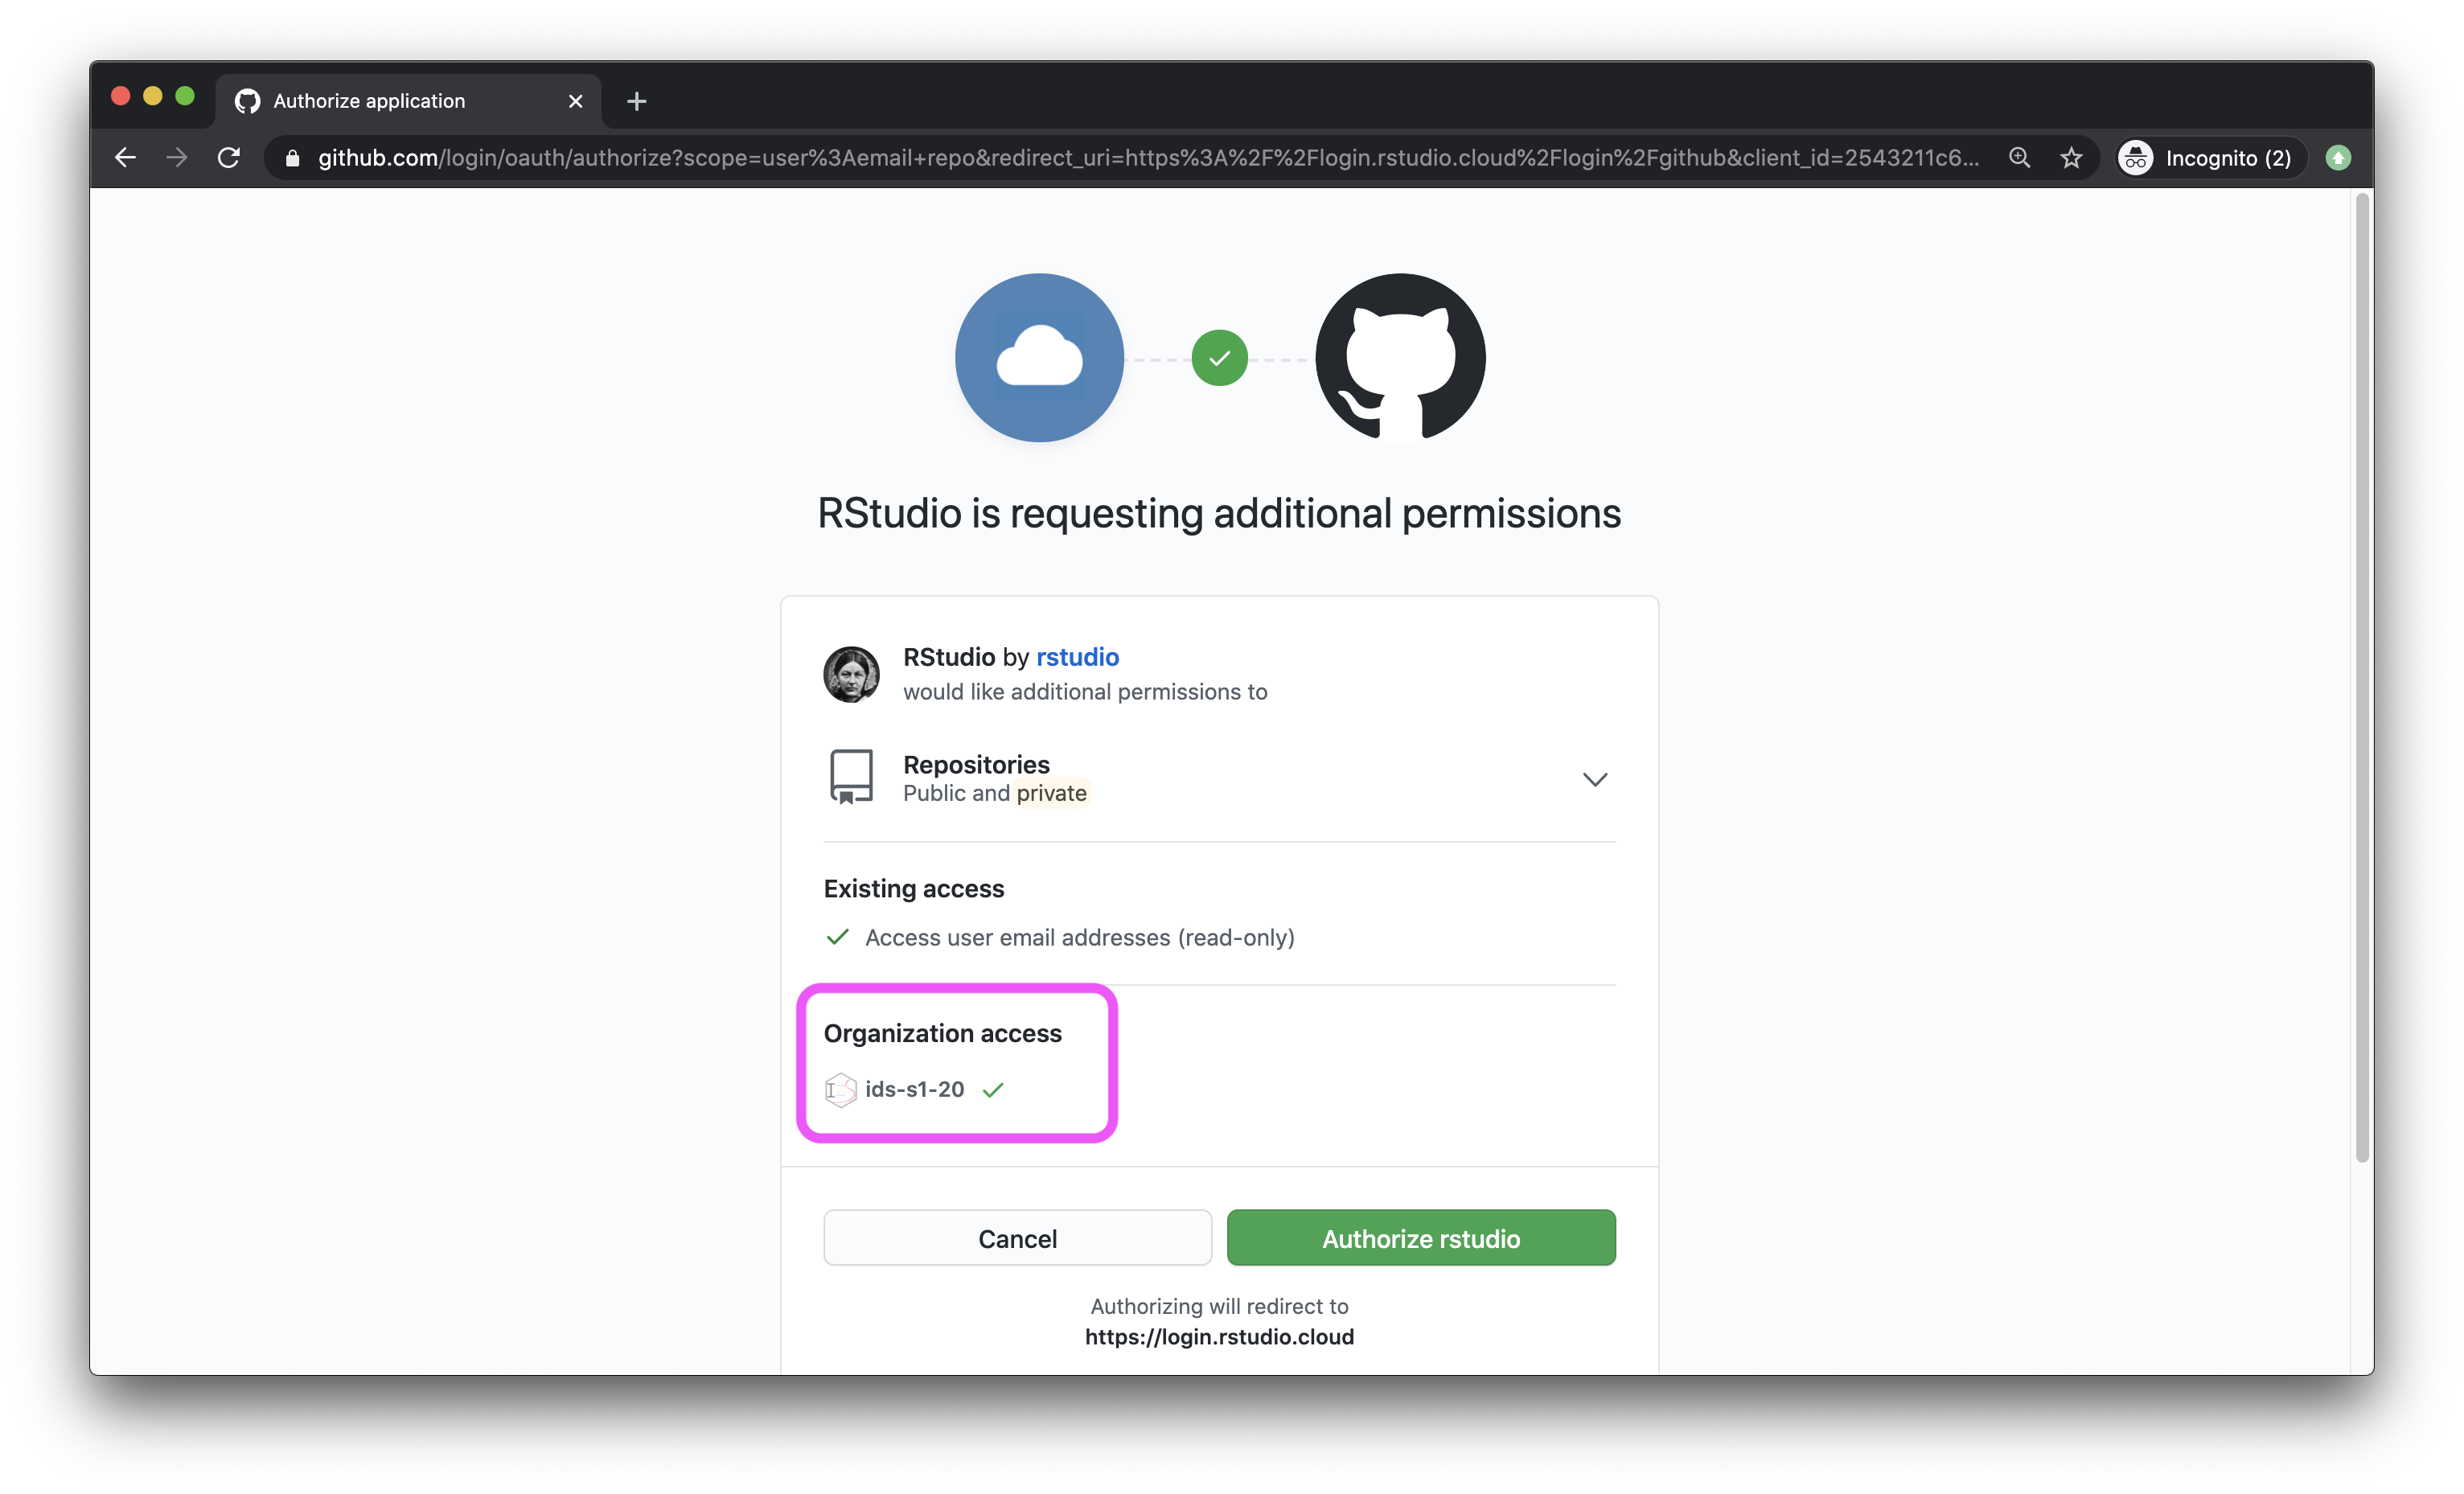
\includegraphics[keepaspectratio]{img/github-auth-4.png}}

\begin{itemize}
\tightlist
\item
  Once you're done, both of these boxes should be checked.
\end{itemize}

\pandocbounded{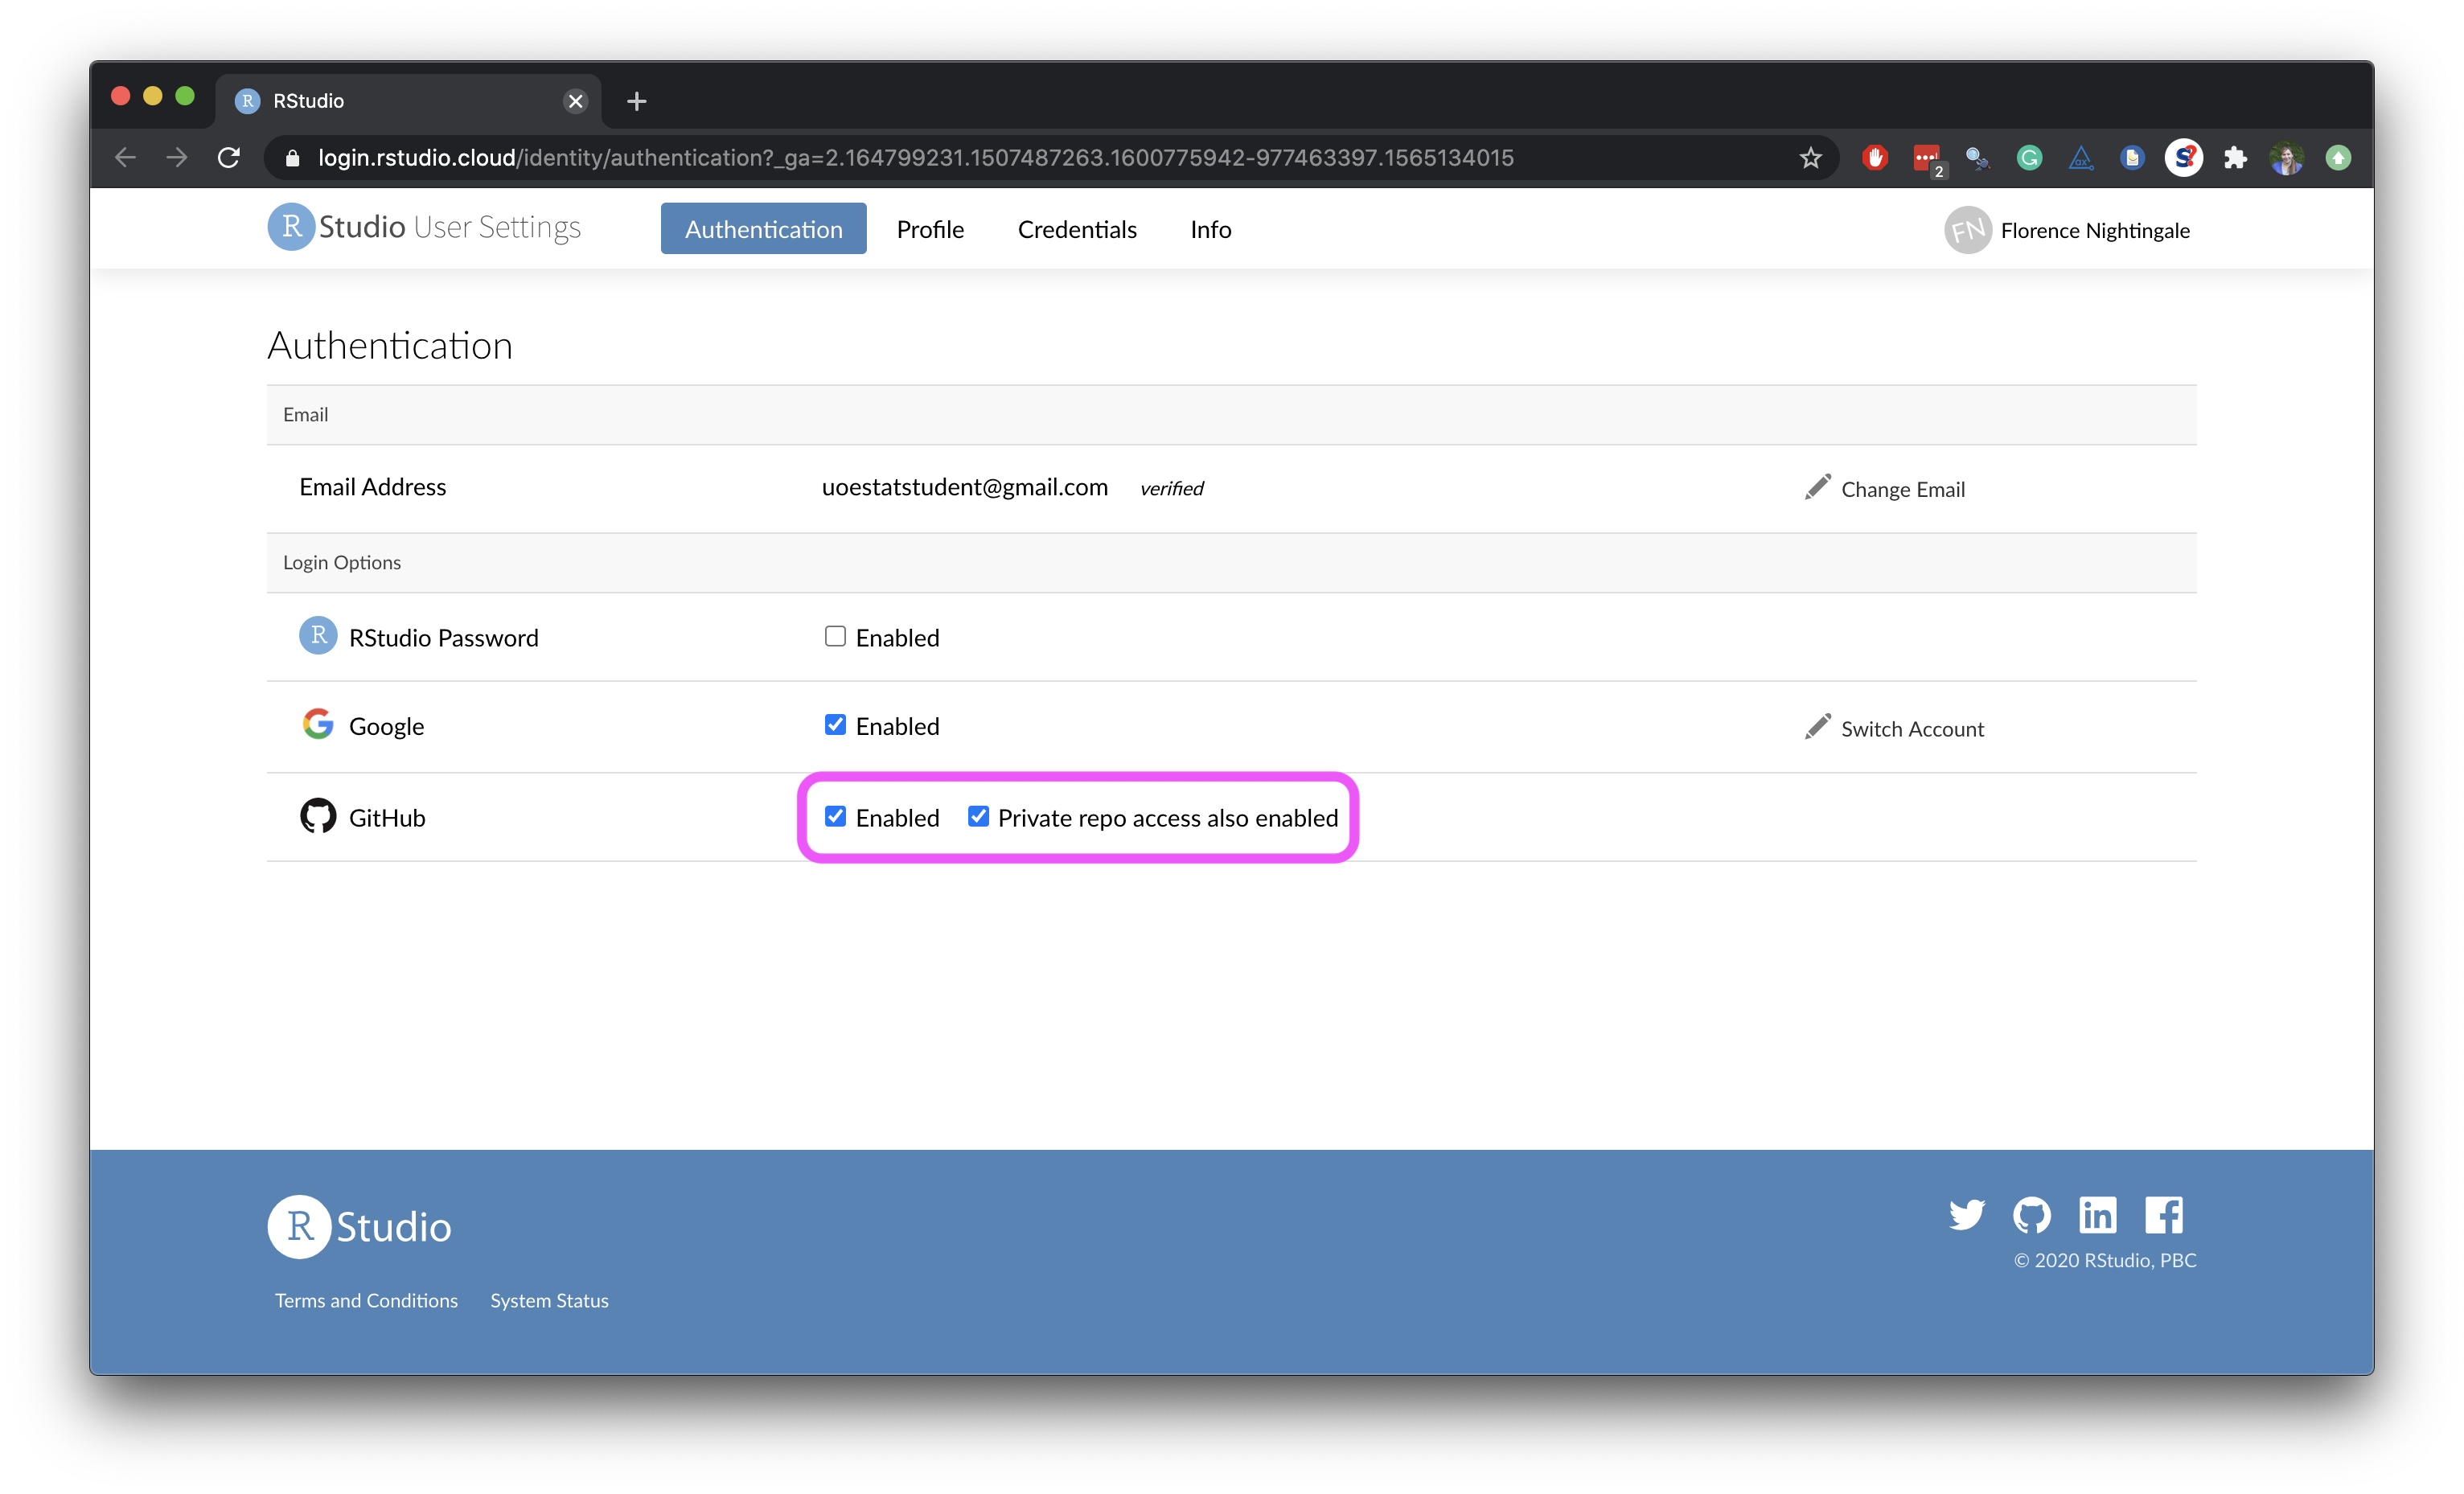
\includegraphics[keepaspectratio]{img/github-auth-5.png}}

\begin{itemize}
\tightlist
\item
  To confirm that you've successfully linked up your GitHub and RStudio
  Cloud accounts, \href{https://github.com/settings/applications}{GitHub
  settings \textgreater{} Applications}. You should see RStudio listed
  as an authorized app under \emph{Authorized OAuth Apps}. If you don't
  this is a good time to ask a question.
\end{itemize}

\pandocbounded{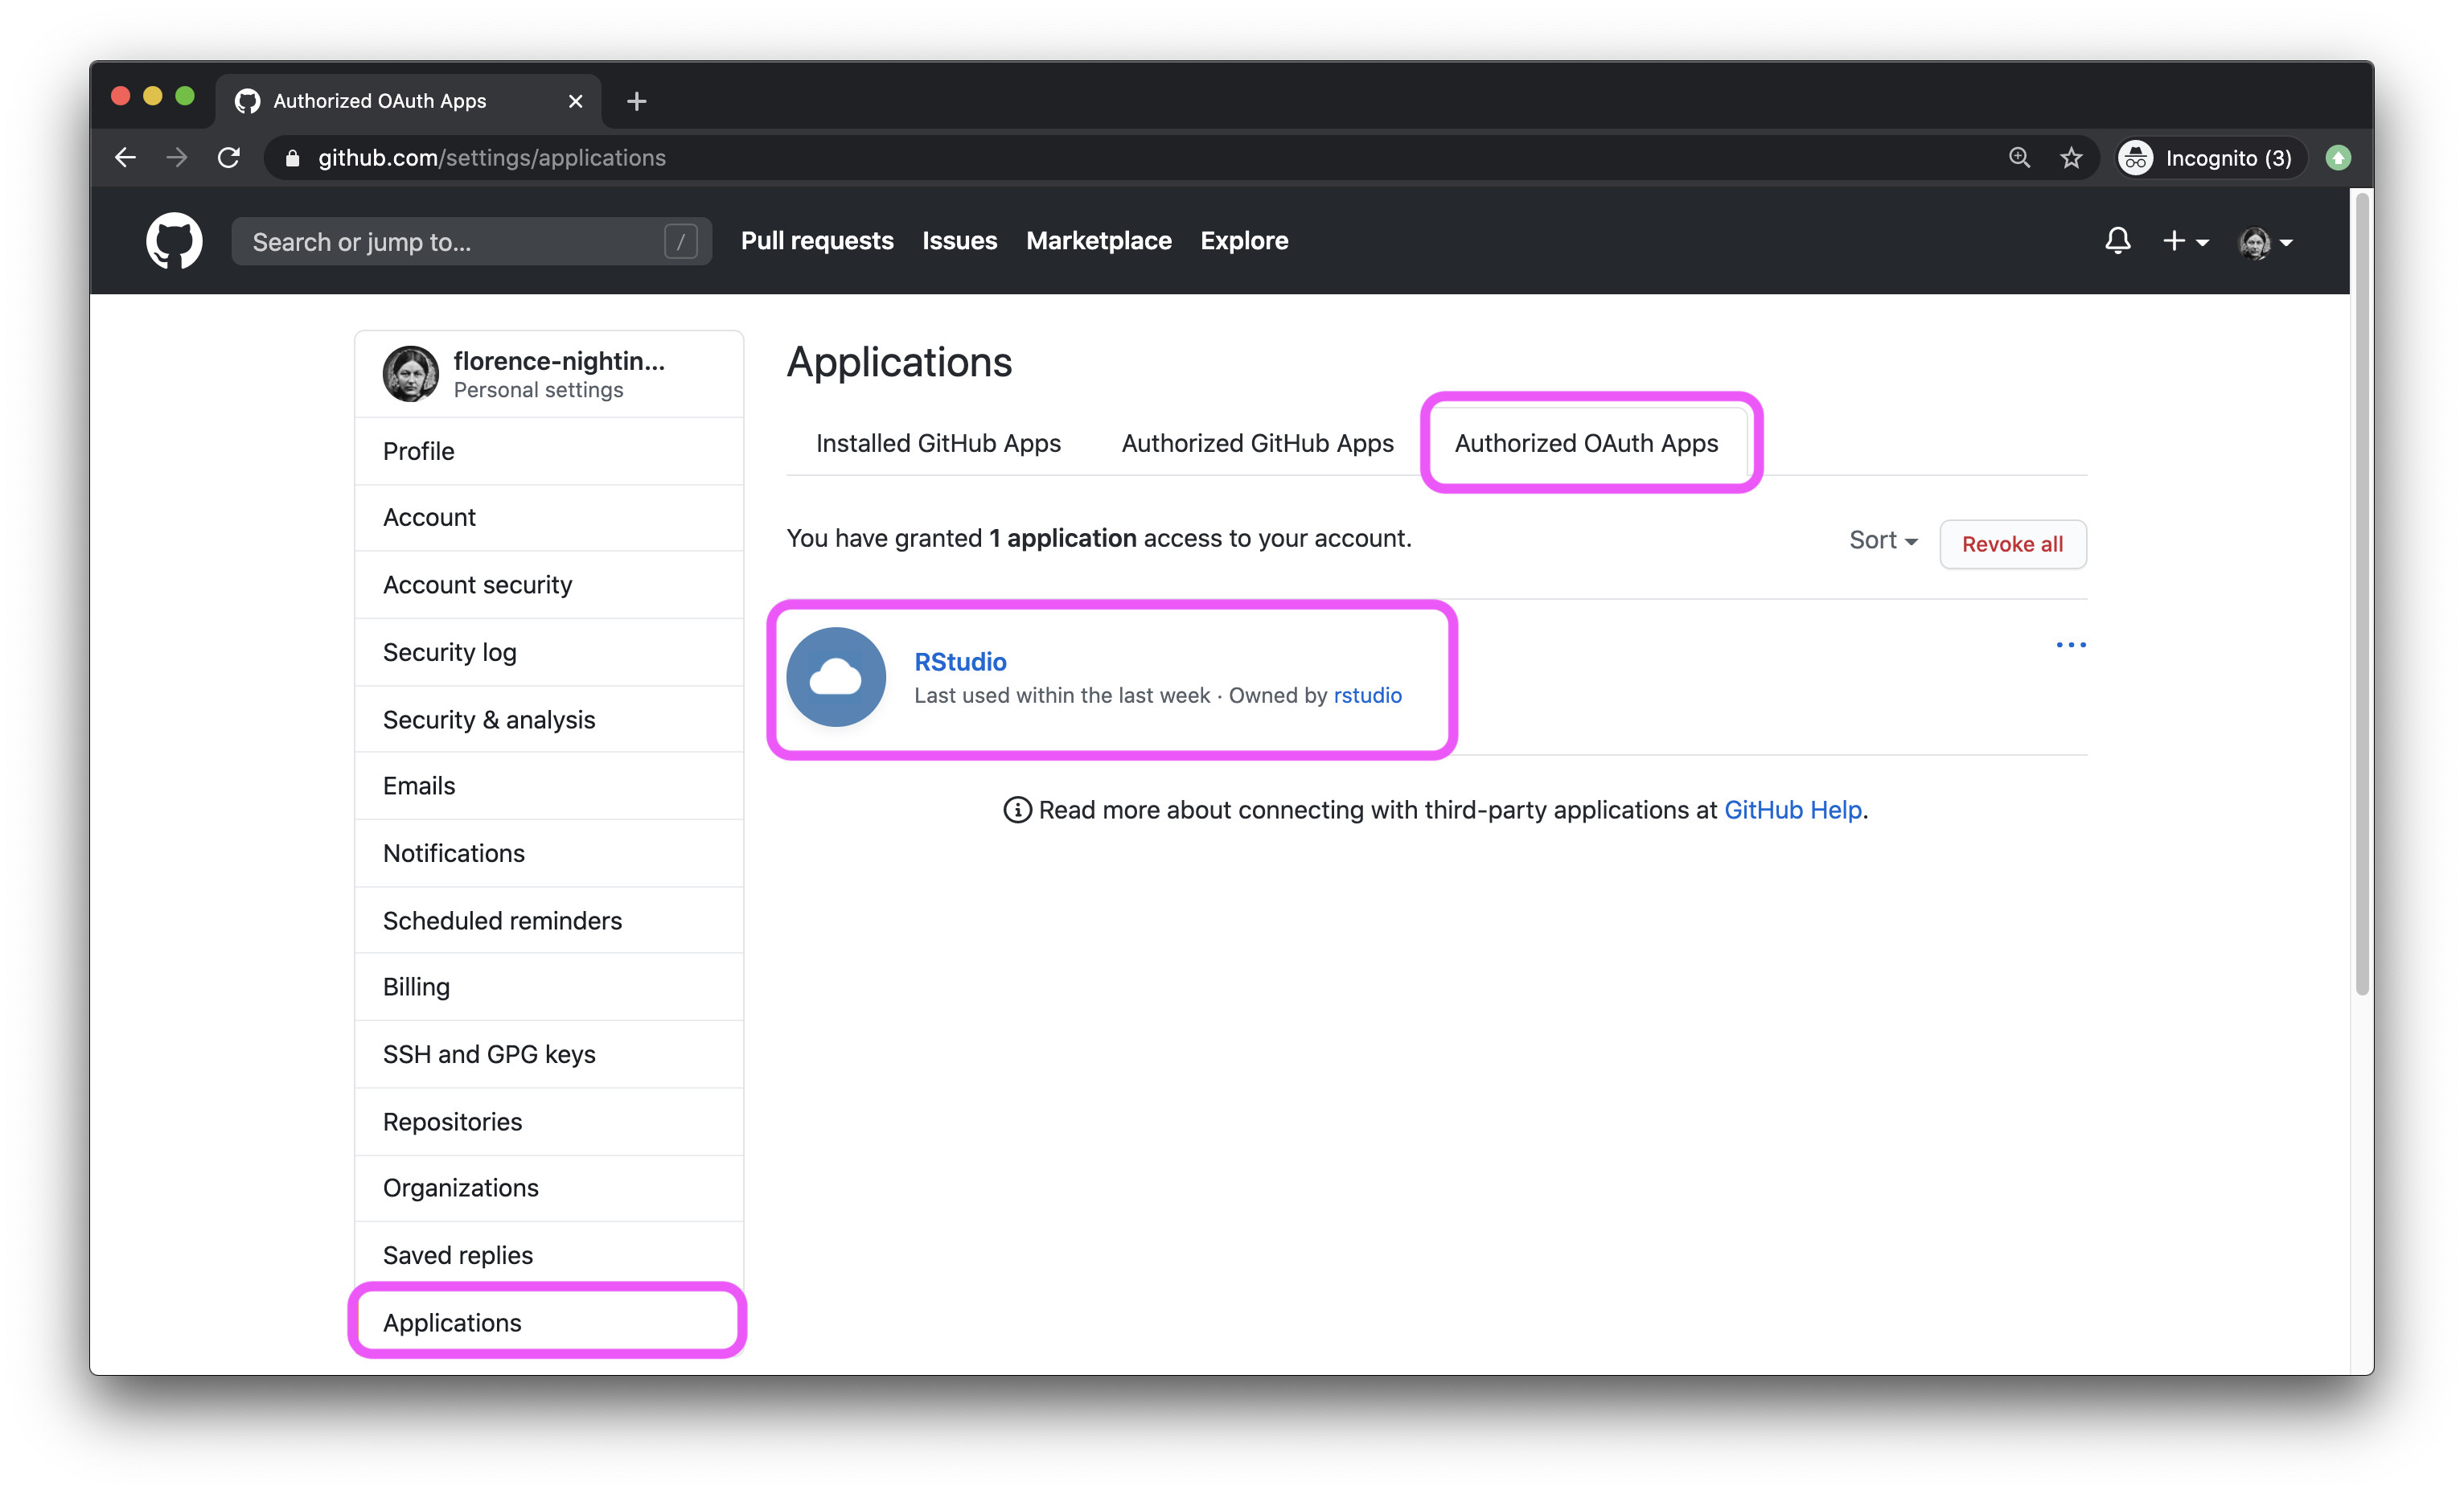
\includegraphics[keepaspectratio]{img/github-auth-6.png}}

\section{Getting started}\label{getting-started}

Each of your assignments will begin with the following steps. You saw
these once in class yesterday, they're outlined in detail here again.
Going forward each lab will start with a ``Getting started'' section but
details will be a bit more sparse than this. You can always refer back
to this lab for a detailed list of the steps involved for getting
started with an assignment.

\begin{itemize}
\tightlist
\item
  Click on the assignment link that you should have received in your
  email to create your GitHub repository (which we'll refer to as
  ``repo'' going forward) for the assignment. This repo contains a
  template you can build on to complete your assignment.
\end{itemize}

\pandocbounded{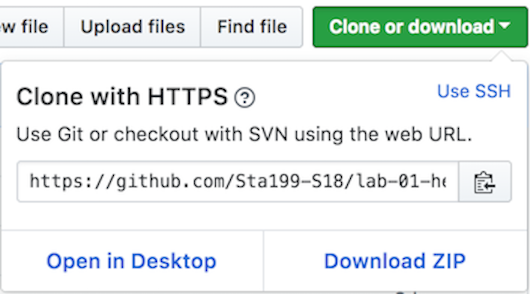
\includegraphics[keepaspectratio]{img/clone-repo-link.png}}

\begin{itemize}
\tightlist
\item
  On GitHub, click on the green \textbf{Clone or download} button,
  select \textbf{Use HTTPS} (this might already be selected by default,
  and if it is, you'll see the text \textbf{Clone with HTTPS} as in the
  image below). Click on the clipboard icon to copy the repo URL.
\end{itemize}

\pandocbounded{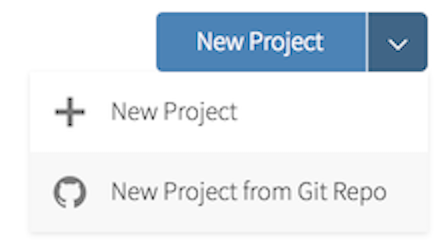
\includegraphics[keepaspectratio]{img/new-project-from-gh.png}}

\begin{itemize}
\tightlist
\item
  Go to RStudio Cloud and into the course workspace. Create a
  \textbf{New Project from Git Repo}. You will need to click on the down
  arrow next to the \textbf{New Project} button to see this option.
\end{itemize}

\pandocbounded{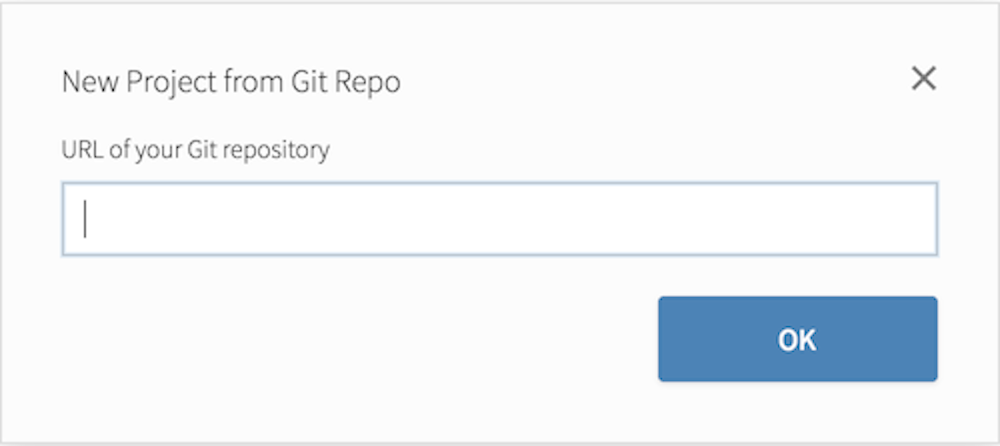
\includegraphics[keepaspectratio]{img/paste-gh-repo-url.png}}

\begin{itemize}
\item
  Copy and paste the URL of your assignment repo into the dialog box:
\item
  Hit OK, and you're good to go!
\end{itemize}

\subsection{Warm up}\label{warm-up}

Before we introduce the data, let's warm up with some simple exercises.

\begin{Shaded}
\begin{Highlighting}[]
\NormalTok{The top portion of your R Markdown file (between the three dashed lines) is called YAML. It stands for "YAML Ain\textquotesingle{}t Markup Language". It is a human friendly data serialization standard for all programming languages. All you need to know is that this area is called the YAML (we will refer to it as such) and that it contains meta information about your document.}
\end{Highlighting}
\end{Shaded}

\subsubsection{YAML}\label{yaml}

Open the R Markdown (Rmd) file in your project, change the author name
to your name, and knit the document.

\pandocbounded{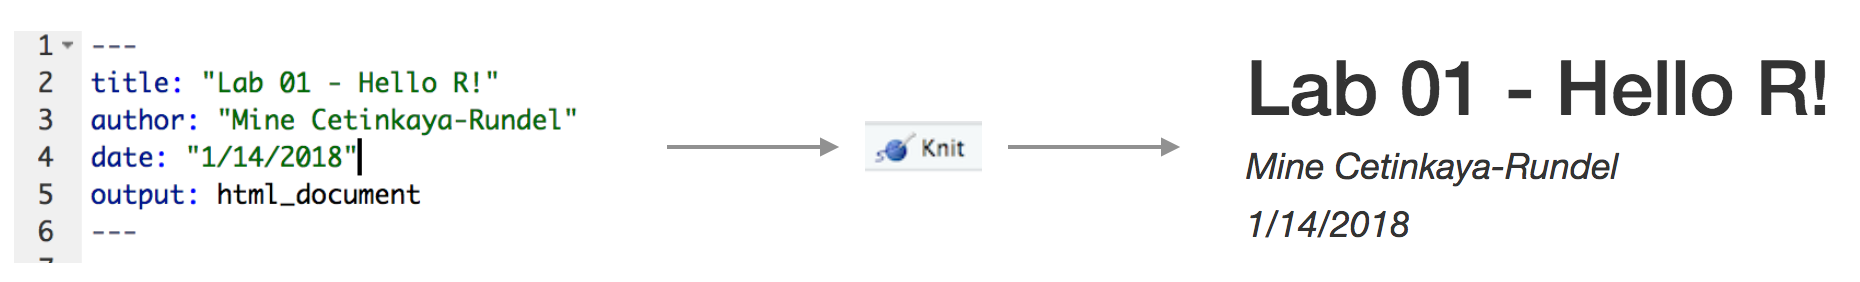
\includegraphics[keepaspectratio]{img/yaml-raw-to-rendered.png}}

\subsubsection{Committing changes}\label{committing-changes}

Then go to the Git pane in your RStudio.

If you have made changes to your Rmd file, you should see it listed
here. Click on it to select it in this list and then click on
\textbf{Diff}. This shows you the \emph{diff}erence between the last
committed state of the document and its current state that includes your
changes. If you're happy with these changes, write ``Update author
name'' in the \textbf{Commit message} box and hit \textbf{Commit}.

\pandocbounded{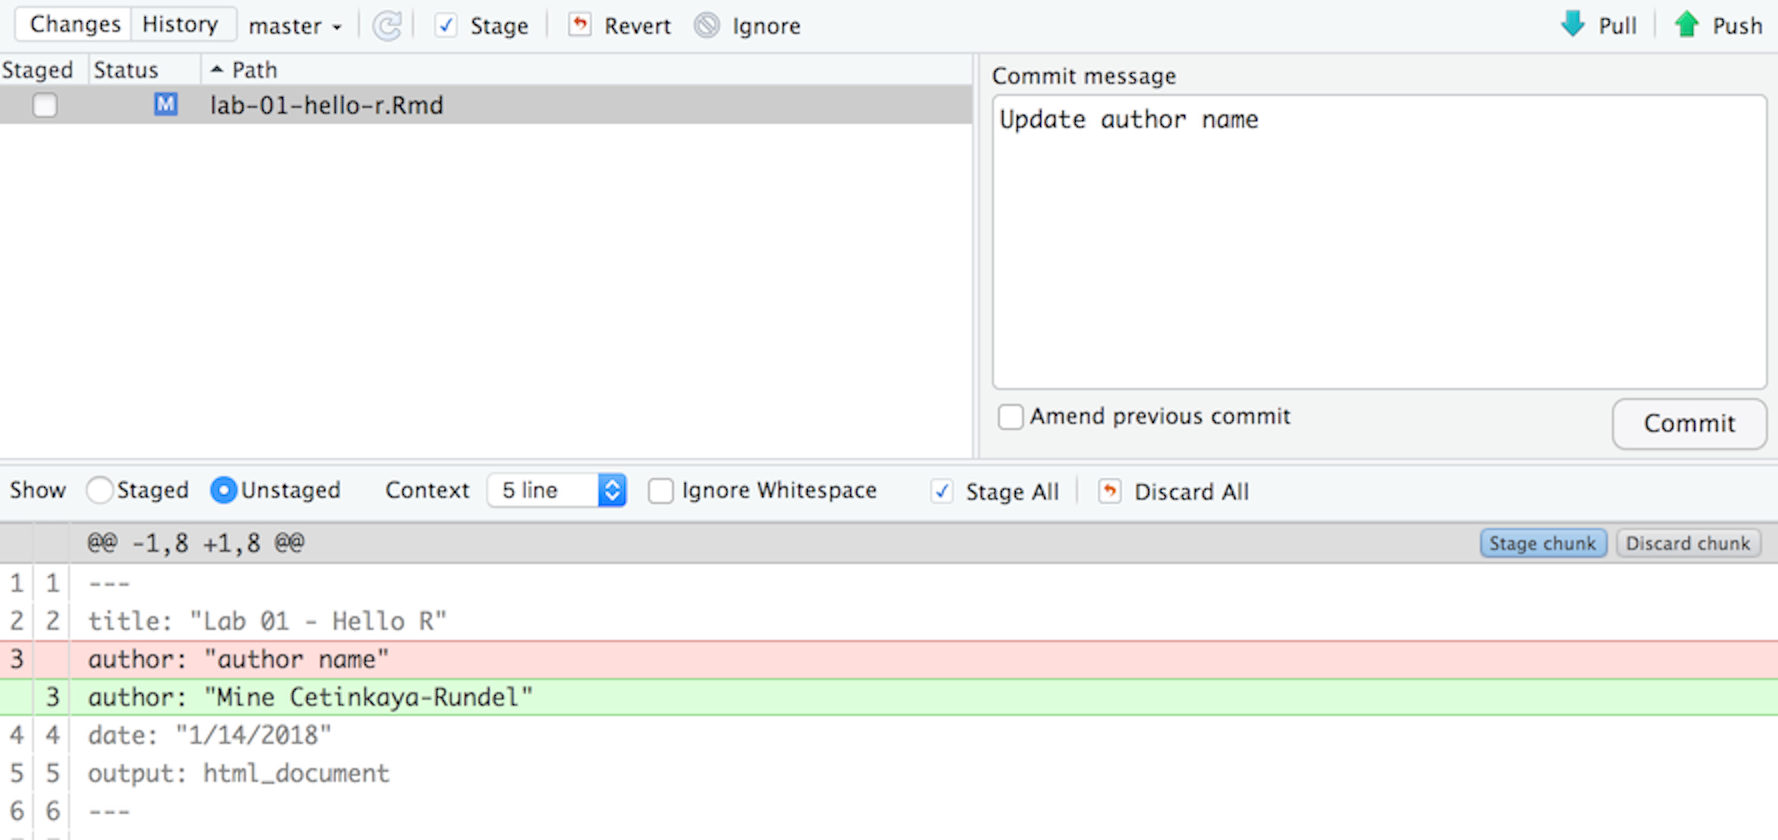
\includegraphics[keepaspectratio]{img/update-author-name-commit.png}}

You don't have to commit after every change, this would get quite
cumbersome. You should consider committing states that are
\emph{meaningful to you} for inspection, comparison, or restoration. In
the first few assignments we will tell you exactly when to commit and in
some cases, what commit message to use. As the semester progresses we
will let you make these decisions.

\subsubsection{Pushing changes}\label{pushing-changes}

Now that you have made an update and committed this change, it's time to
push these changes to the web! Or more specifically, to your repo on
GitHub. Why? So that others can see your changes. And by others, we mean
the course teaching team (your repos in this course are private to you
and us, only).

In order to push your changes to GitHub, click on \textbf{Push}. This
will prompt a dialogue box where you first need to enter your user name,
and then your password. This might feel cumbersome. Bear with me\ldots{}
We \emph{will} teach you how to save your password so you don't have to
enter it every time. But for this one assignment you'll have to manually
enter each time you push in order to gain some experience with it.

\subsection{Packages}\label{packages}

In this lab we will work with two packages: \textbf{datasauRus} which
contains the dataset we'll be using and \textbf{tidyverse} which is a
collection of packages for doing data analysis in a ``tidy'' way. These
packages are already installed for you. You can load the packages by
running the following in the Console.

\begin{Shaded}
\begin{Highlighting}[]
\FunctionTok{library}\NormalTok{(tidyverse) }
\FunctionTok{library}\NormalTok{(datasauRus)}
\end{Highlighting}
\end{Shaded}

Note that the packages are also loaded with the same commands in your R
Markdown document.

\subsection{Data}\label{data}

\begin{Shaded}
\begin{Highlighting}[]
\NormalTok{If it\textquotesingle{}s confusing that the data frame is called \textasciigrave{}datasaurus\_dozen\textasciigrave{} when it contains 13 datasets, you\textquotesingle{}re not alone! Have you heard of a [baker\textquotesingle{}s dozen](https://en.wikipedia.org/wiki/Dozen\#Baker\textquotesingle{}s\_dozen)?}
\end{Highlighting}
\end{Shaded}

The data frame we will be working with today is called
\texttt{datasaurus\_dozen} and it's in the \texttt{datasauRus} package.
Actually, this single data frame contains 13 datasets, designed to show
us why data visualisation is important and how summary statistics alone
can be misleading. The different datasets are marked by the
\texttt{dataset} variable.

To find out more about the dataset, type the following in your Console:
\texttt{?datasaurus\_dozen}. A question mark before the name of an
object will always bring up its help file. This command must be ran in
the Console.

\section{Exercises}\label{exercises}

\begin{enumerate}
\def\labelenumi{\arabic{enumi}.}
\tightlist
\item
  Based on the help file, how many rows and how many columns does the
  \texttt{datasaurus\_dozen} file have? What are the variables included
  in the data frame? Add your responses to your lab report.
\end{enumerate}

According to the help file, the \texttt{datasaurus\_dozen} dataset has
1846 rows and 3 columns. The variables included in the data frame are: -
\texttt{dataset}: The name of the dataset - \texttt{x}: x-coordinate
value - \texttt{y}: y-coordinate value

Let's take a look at what these datasets are. To do so we can make a
\emph{frequency table} of the dataset variable:

\begin{Shaded}
\begin{Highlighting}[]
\NormalTok{datasaurus\_dozen }\SpecialCharTok{\%\textgreater{}\%}
  \FunctionTok{count}\NormalTok{(dataset) }\SpecialCharTok{\%\textgreater{}\%}
  \FunctionTok{print}\NormalTok{(}\DecValTok{13}\NormalTok{)}
\end{Highlighting}
\end{Shaded}

\begin{verbatim}
## # A tibble:
## #   13 x 2
##    dataset   
##    <chr>     
##  1 away      
##  2 bullseye  
##  3 circle    
##  4 dino      
##  5 dots      
##  6 h_lines   
##  7 high_lines
##  8 slant_down
##  9 slant_up  
## 10 star      
## 11 v_lines   
## 12 wide_lines
## 13 x_shape   
## # i 1 more
## #   variable:
## #   n <int>
\end{verbatim}

\begin{Shaded}
\begin{Highlighting}[]
\NormalTok{Matejka, Justin, and George Fitzmaurice. "Same stats, different graphs: Generating datasets with varied appearance and identical statistics through simulated annealing." Proceedings of the 2017 CHI Conference on Human Factors in Computing Systems. ACM, 2017.}
\end{Highlighting}
\end{Shaded}

The original Datasaurus (\texttt{dino}) was created by Alberto Cairo in
\href{http://www.thefunctionalart.com/2016/08/download-datasaurus-never-trust-summary.html}{this
great blog post}. The other Dozen were generated using simulated
annealing and the process is described in the paper \emph{Same Stats,
Different Graphs: Generating Datasets with Varied Appearance and
Identical Statistics} through Simulated Annealing by Justin Matejka and
George Fitzmaurice. In the paper, the authors simulate a variety of
datasets that have the same summary statistics as the Datasaurus but
have very different distributions.

🧶 ✅ ⬆️ \emph{Knit, commit, and push your changes to GitHub with the
commit message ``Added answer for Ex 1''. Make sure to commit and push
all changed files so that your Git pane is cleared up afterwards.}

\begin{enumerate}
\def\labelenumi{\arabic{enumi}.}
\setcounter{enumi}{1}
\tightlist
\item
  Plot \texttt{y} vs.~\texttt{x} for the \texttt{dino} dataset. Then,
  calculate the correlation coefficient between \texttt{x} and
  \texttt{y} for this dataset.
\end{enumerate}

Below is the code you will need to complete this exercise. Basically,
the answer is already given, but you need to include relevant bits in
your Rmd document and successfully knit it and view the results.

Start with the \texttt{datasaurus\_dozen} and pipe it into the
\texttt{filter} function to filter for observations where
\texttt{dataset\ ==\ "dino"}. Store the resulting filtered data frame as
a new data frame called \texttt{dino\_data}.

\begin{Shaded}
\begin{Highlighting}[]
\NormalTok{dino\_data }\OtherTok{\textless{}{-}}\NormalTok{ datasaurus\_dozen }\SpecialCharTok{\%\textgreater{}\%}
  \FunctionTok{filter}\NormalTok{(dataset }\SpecialCharTok{==} \StringTok{"dino"}\NormalTok{)}
\end{Highlighting}
\end{Shaded}

There is a lot going on here, so let's slow down and unpack it a bit.

First, the pipe operator: \texttt{\%\textgreater{}\%}, takes what comes
before it and sends it as the first argument to what comes after it. So
here, we're saying \texttt{filter} the \texttt{datasaurus\_dozen} data
frame for observations where \texttt{dataset\ ==\ "dino"}.

Second, the assignment operator: \texttt{\textless{}-}, assigns the name
\texttt{dino\_data} to the filtered data frame.

Next, we need to visualize these data. We will use the \texttt{ggplot}
function for this. Its first argument is the data you're visualizing.
Next we define the \texttt{aes}thetic mappings. In other words, the
columns of the data that get mapped to certain aesthetic features of the
plot, e.g.~the \texttt{x} axis will represent the variable called
\texttt{x} and the \texttt{y} axis will represent the variable called
\texttt{y}. Then, we add another layer to this plot where we define
which \texttt{geom}etric shapes we want to use to represent each
observation in the data. In this case we want these to be points, hence
\texttt{geom\_point}.

\begin{Shaded}
\begin{Highlighting}[]
\FunctionTok{ggplot}\NormalTok{(}\AttributeTok{data =}\NormalTok{ dino\_data, }\AttributeTok{mapping =} \FunctionTok{aes}\NormalTok{(}\AttributeTok{x =}\NormalTok{ x, }\AttributeTok{y =}\NormalTok{ y)) }\SpecialCharTok{+}
  \FunctionTok{geom\_point}\NormalTok{()}
\end{Highlighting}
\end{Shaded}

\pandocbounded{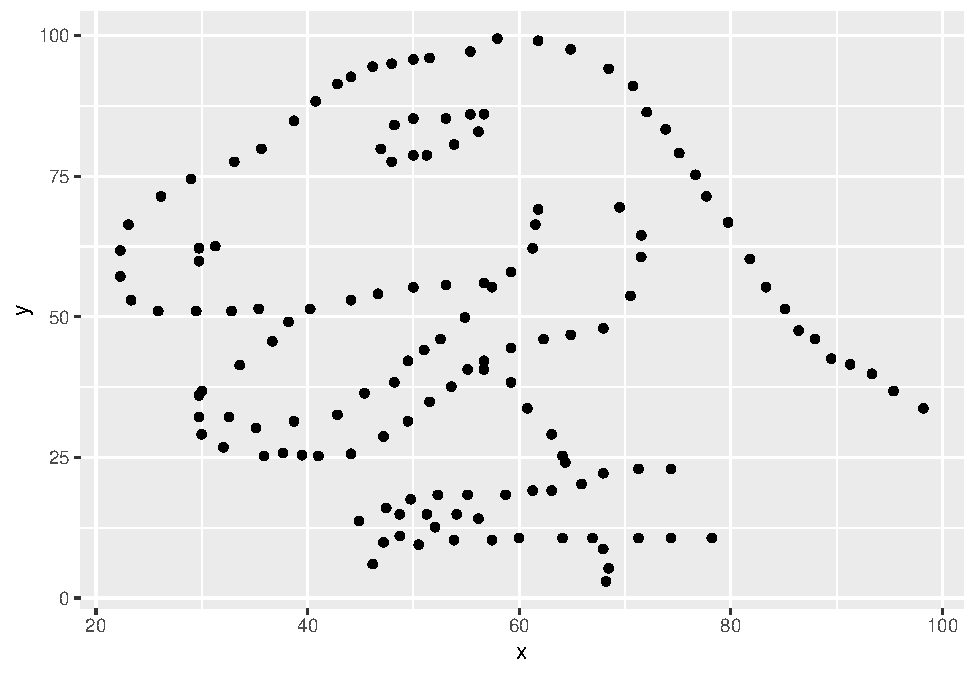
\includegraphics[keepaspectratio]{lab-01-hello-r_files/figure-latex/unnamed-chunk-9-1.pdf}}

If this seems like a lot, it is. And you will learn about the philosophy
of building data visualizations in layer in detail next week. For now,
follow along with the code that is provided.

For the second part of these exercises, we need to calculate a summary
statistic: the correlation coefficient. Correlation coefficient, often
referred to as \(r\) in statistics, measures the linear association
between two variables. You will see that some of the pairs of variables
we plot do not have a linear relationship between them. This is exactly
why we want to visualize first: visualize to assess the form of the
relationship, and calculate \(r\) only if relevant. In this case,
calculating a correlation coefficient really doesn't make sense since
the relationship between \texttt{x} and \texttt{y} is definitely not
linear -- it's dinosaurial!

But, for illustrative purposes, let's calculate the correlation
coefficient between \texttt{x} and \texttt{y}.

\begin{Shaded}
\begin{Highlighting}[]
\NormalTok{Start with \textasciigrave{}dino\_data\textasciigrave{} and calculate a summary statistic that we will call \textasciigrave{}r\textasciigrave{} as the \textasciigrave{}cor\textasciigrave{}relation between \textasciigrave{}x\textasciigrave{} and \textasciigrave{}y\textasciigrave{}.}
\end{Highlighting}
\end{Shaded}

\begin{Shaded}
\begin{Highlighting}[]
\NormalTok{dino\_data }\SpecialCharTok{\%\textgreater{}\%}
  \FunctionTok{summarize}\NormalTok{(}\AttributeTok{r =} \FunctionTok{cor}\NormalTok{(x, y))}
\end{Highlighting}
\end{Shaded}

\begin{verbatim}
## # A tibble: 1 x 1
##         r
##     <dbl>
## 1 -0.0645
\end{verbatim}

Based on the plot, we can see that the points form the shape of a
dinosaur. The correlation coefficient between \texttt{x} and \texttt{y}
for the \texttt{dino} dataset is approximately -0.065, which is very
close to zero. This suggests that there is almost no linear relationship
between the variables, even though the visualization clearly shows a
pattern.

🧶 ✅ ⬆️ \emph{Knit, commit, and push your changes to GitHub with the
commit message ``Added answer for Ex 2''. Make sure to commit and push
all changed files so that your Git pane is cleared up afterwards.}

\begin{enumerate}
\def\labelenumi{\arabic{enumi}.}
\setcounter{enumi}{2}
\tightlist
\item
  Plot \texttt{y} vs.~\texttt{x} for the \texttt{star} dataset. You can
  (and should) reuse code we introduced above, just replace the dataset
  name with the desired dataset. Then, calculate the correlation
  coefficient between \texttt{x} and \texttt{y} for this dataset. How
  does this value compare to the \texttt{r} of \texttt{dino}?
\end{enumerate}

\begin{Shaded}
\begin{Highlighting}[]
\NormalTok{star\_data }\OtherTok{\textless{}{-}}\NormalTok{ datasaurus\_dozen }\SpecialCharTok{\%\textgreater{}\%}
  \FunctionTok{filter}\NormalTok{(dataset }\SpecialCharTok{==} \StringTok{"star"}\NormalTok{)}

\FunctionTok{ggplot}\NormalTok{(}\AttributeTok{data =}\NormalTok{ star\_data, }\AttributeTok{mapping =} \FunctionTok{aes}\NormalTok{(}\AttributeTok{x =}\NormalTok{ x, }\AttributeTok{y =}\NormalTok{ y)) }\SpecialCharTok{+}
  \FunctionTok{geom\_point}\NormalTok{()}
\end{Highlighting}
\end{Shaded}

\pandocbounded{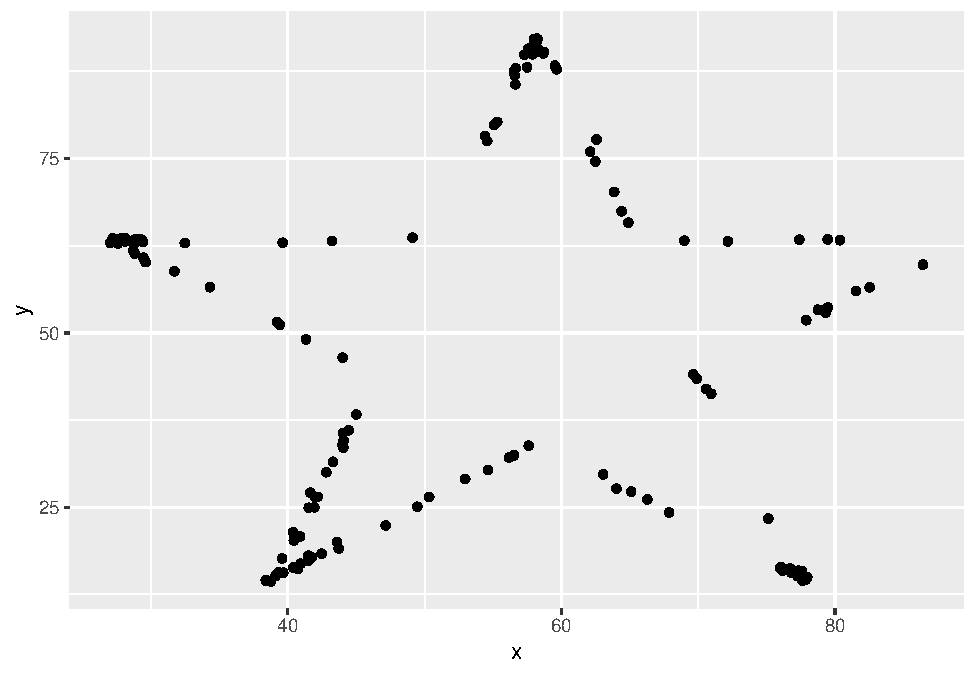
\includegraphics[keepaspectratio]{lab-01-hello-r_files/figure-latex/unnamed-chunk-12-1.pdf}}

\begin{Shaded}
\begin{Highlighting}[]
\NormalTok{star\_data }\SpecialCharTok{\%\textgreater{}\%}
  \FunctionTok{summarize}\NormalTok{(}\AttributeTok{r =} \FunctionTok{cor}\NormalTok{(x, y))}
\end{Highlighting}
\end{Shaded}

\begin{verbatim}
## # A tibble: 1 x 1
##         r
##     <dbl>
## 1 -0.0630
\end{verbatim}

The correlation coefficient for the \texttt{star} dataset is
approximately -0.063, which is very similar to the \texttt{r} of
\texttt{dino} (-0.065). Despite having almost identical correlation
coefficients, the visual patterns in the two datasets are completely
different. This demonstrates how summary statistics alone can be
misleading.

🧶 ✅ ⬆️ \emph{This is another good place to pause, knit, commit changes
with the commit message ``Added answer for Ex 3'', and push. Make sure
to commit and push all changed files so that your Git pane is cleared up
afterwards.}

\begin{enumerate}
\def\labelenumi{\arabic{enumi}.}
\setcounter{enumi}{3}
\tightlist
\item
  Plot \texttt{y} vs.~\texttt{x} for the \texttt{circle} dataset. You
  can (and should) reuse code we introduced above, just replace the
  dataset name with the desired dataset. Then, calculate the correlation
  coefficient between \texttt{x} and \texttt{y} for this dataset. How
  does this value compare to the \texttt{r} of \texttt{dino}?
\end{enumerate}

\begin{Shaded}
\begin{Highlighting}[]
\NormalTok{circle\_data }\OtherTok{\textless{}{-}}\NormalTok{ datasaurus\_dozen }\SpecialCharTok{\%\textgreater{}\%}
  \FunctionTok{filter}\NormalTok{(dataset }\SpecialCharTok{==} \StringTok{"circle"}\NormalTok{)}

\FunctionTok{ggplot}\NormalTok{(}\AttributeTok{data =}\NormalTok{ circle\_data, }\AttributeTok{mapping =} \FunctionTok{aes}\NormalTok{(}\AttributeTok{x =}\NormalTok{ x, }\AttributeTok{y =}\NormalTok{ y)) }\SpecialCharTok{+}
  \FunctionTok{geom\_point}\NormalTok{()}
\end{Highlighting}
\end{Shaded}

\pandocbounded{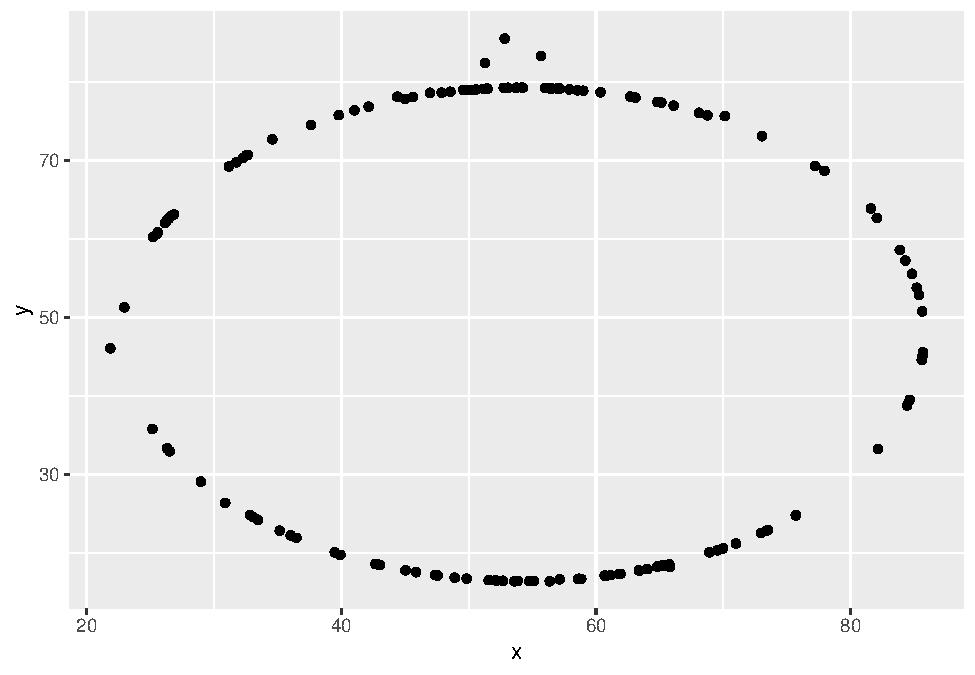
\includegraphics[keepaspectratio]{lab-01-hello-r_files/figure-latex/unnamed-chunk-13-1.pdf}}

\begin{Shaded}
\begin{Highlighting}[]
\NormalTok{circle\_data }\SpecialCharTok{\%\textgreater{}\%}
  \FunctionTok{summarize}\NormalTok{(}\AttributeTok{r =} \FunctionTok{cor}\NormalTok{(x, y))}
\end{Highlighting}
\end{Shaded}

\begin{verbatim}
## # A tibble: 1 x 1
##         r
##     <dbl>
## 1 -0.0683
\end{verbatim}

The correlation coefficient for the \texttt{circle} dataset is
approximately -0.068, which is again very similar to the \texttt{r}
values of both \texttt{dino} (-0.065) and \texttt{star} (-0.063).
Despite having nearly identical correlation coefficients, the visual
pattern is completely different from both previous datasets. This
further illustrates the importance of visualizing your data rather than
relying solely on summary statistics.

🧶 ✅ ⬆️ \emph{You should pause again, commit changes with the commit
message ``Added answer for Ex 4'', and push. Make sure to commit and
push all changed files so that your Git pane is cleared up afterwards.}

\begin{Shaded}
\begin{Highlighting}[]
\NormalTok{Facet by the dataset variable, placing the plots in a 3 column grid, and don\textquotesingle{}t add a legend.}
\end{Highlighting}
\end{Shaded}

\begin{enumerate}
\def\labelenumi{\arabic{enumi}.}
\setcounter{enumi}{4}
\tightlist
\item
  Finally, let's plot all datasets at once. In order to do this we will
  make use of faceting.
\end{enumerate}

\begin{Shaded}
\begin{Highlighting}[]
\FunctionTok{ggplot}\NormalTok{(datasaurus\_dozen, }\FunctionTok{aes}\NormalTok{(}\AttributeTok{x =}\NormalTok{ x, }\AttributeTok{y =}\NormalTok{ y, }\AttributeTok{color =}\NormalTok{ dataset))}\SpecialCharTok{+}
  \FunctionTok{geom\_point}\NormalTok{()}\SpecialCharTok{+}
  \FunctionTok{facet\_wrap}\NormalTok{(}\SpecialCharTok{\textasciitilde{}}\NormalTok{ dataset, }\AttributeTok{ncol =} \DecValTok{3}\NormalTok{) }\SpecialCharTok{+}
  \FunctionTok{theme}\NormalTok{(}\AttributeTok{legend.position =} \StringTok{"none"}\NormalTok{)}
\end{Highlighting}
\end{Shaded}

\pandocbounded{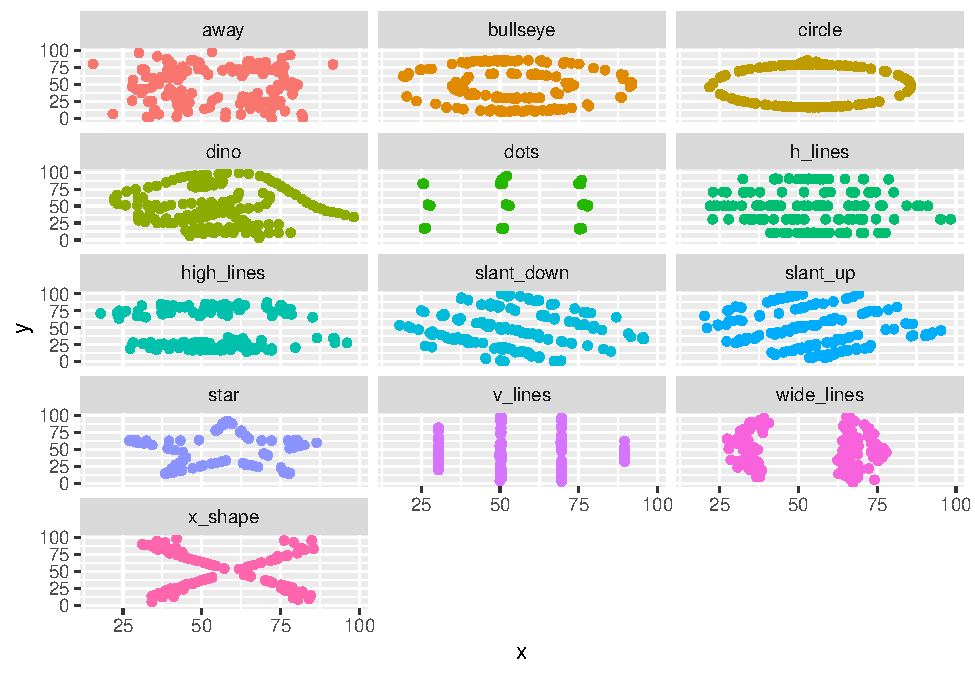
\includegraphics[keepaspectratio]{lab-01-hello-r_files/figure-latex/all-viz-1.pdf}}

And we can use the \texttt{group\_by} function to generate all the
summary correlation coefficients.

\begin{Shaded}
\begin{Highlighting}[]
\NormalTok{datasaurus\_dozen }\SpecialCharTok{\%\textgreater{}\%}
  \FunctionTok{group\_by}\NormalTok{(dataset) }\SpecialCharTok{\%\textgreater{}\%}
  \FunctionTok{summarize}\NormalTok{(}\AttributeTok{r =} \FunctionTok{cor}\NormalTok{(x, y)) }\SpecialCharTok{\%\textgreater{}\%}
  \FunctionTok{print}\NormalTok{(}\DecValTok{13}\NormalTok{)}
\end{Highlighting}
\end{Shaded}

\begin{verbatim}
## # A tibble:
## #   13 x 2
##    dataset   
##    <chr>     
##  1 away      
##  2 bullseye  
##  3 circle    
##  4 dino      
##  5 dots      
##  6 h_lines   
##  7 high_lines
##  8 slant_down
##  9 slant_up  
## 10 star      
## 11 v_lines   
## 12 wide_lines
## 13 x_shape   
## # i 1 more
## #   variable:
## #   r <dbl>
\end{verbatim}

Looking at all the datasets and their correlation coefficients, we can
observe that despite having remarkably similar summary statistics (all
correlations are around -0.06 to -0.07), the visual patterns in the data
are dramatically different. This clearly demonstrates the ``Datasaurus
Dozen'' principle: always visualize your data, as summary statistics can
be identical for datasets with completely different distributions and
patterns.

You're done with the data analysis exercises, but we'd like you to do
two more things:

\pandocbounded{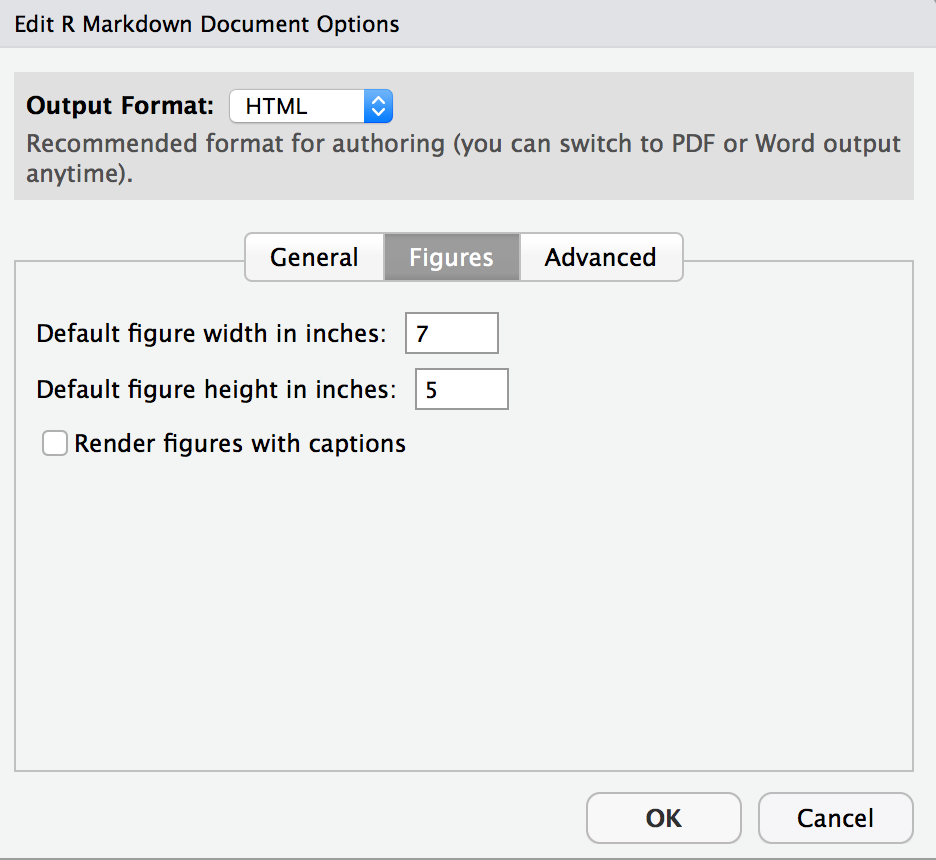
\includegraphics[keepaspectratio]{img/fig-resize-global.png}}

\begin{itemize}
\tightlist
\item
  \textbf{Resize your figures:}
\end{itemize}

Click on the gear icon in on top of the R Markdown document, and select
``Output Options\ldots{}'' in the dropdown menu. In the pop up dialogue
box go to the Figures tab and change the height and width of the
figures, and hit OK when done. Then, knit your document and see how you
like the new sizes. Change and knit again and again until you're happy
with the figure sizes. Note that these values get saved in the YAML.

\pandocbounded{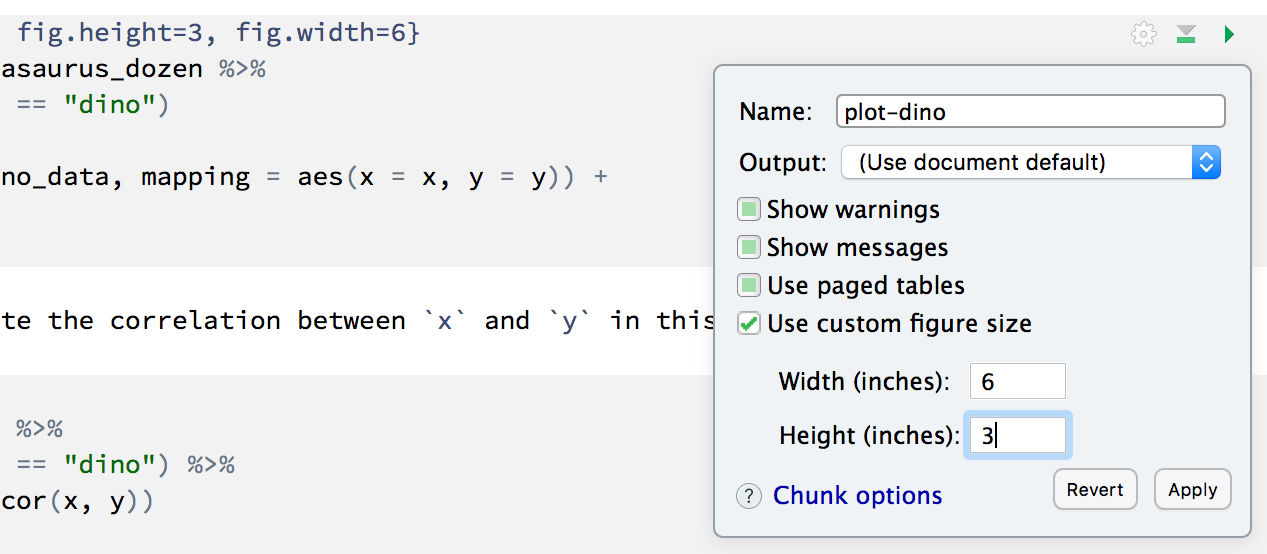
\includegraphics[keepaspectratio]{img/fig-resize-local.png}}

You can also use different figure sizes for differen figures. To do so
click on the gear icon within the chunk where you want to make a change.
Changing the figure sizes added new options to these chunks:
\texttt{fig.width} and \texttt{fig.height}. You can change them by
defining different values directly in your R Markdown document as well.

\pandocbounded{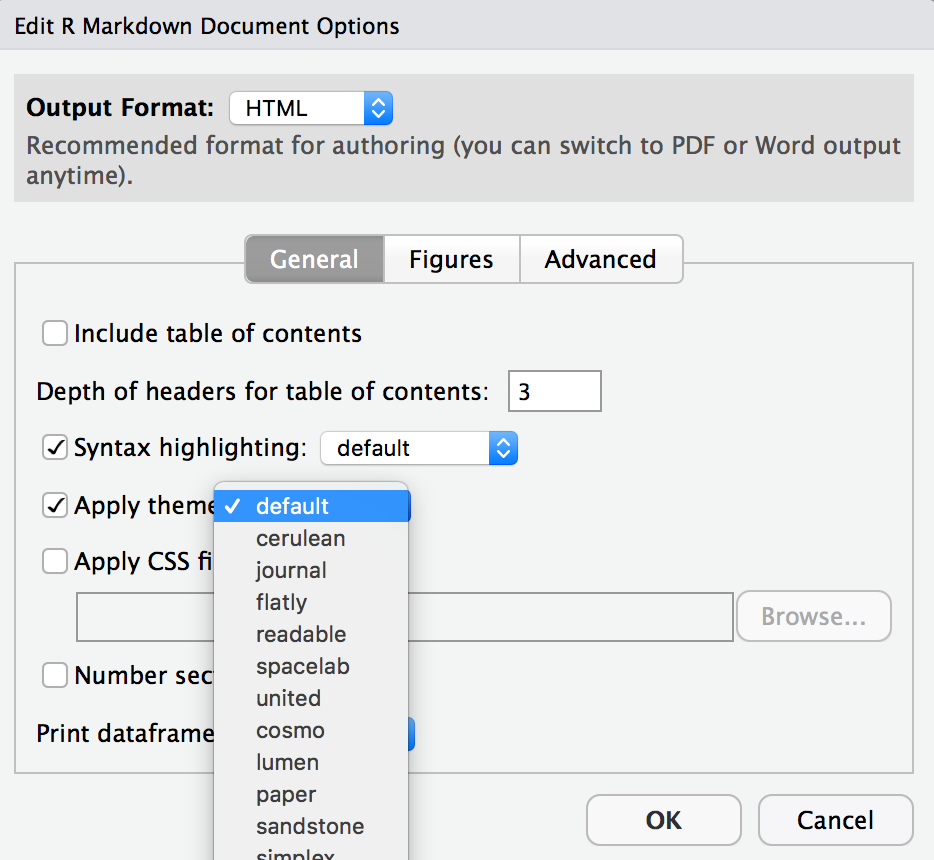
\includegraphics[keepaspectratio]{img/theme-highlight.png}}

\begin{itemize}
\tightlist
\item
  \textbf{Change the look of your report:}
\end{itemize}

Once again click on the gear icon in on top of the R Markdown document,
and select ``Output Options\ldots{}'' in the dropdown menu. In the
General tab of the pop up dialogue box try out different Syntax
highlighting and theme options. Hit OK and knit your document to see how
it looks. Play around with these until you're happy with the look.

\begin{Shaded}
\begin{Highlighting}[]
\NormalTok{Not sure how to use emojis on your computer? Maybe a teammate can help? Or you can ask your TA as well!}
\end{Highlighting}
\end{Shaded}

🧶 ✅ ⬆️ \emph{Yay, you're done! Commit all remaining changes, use the
commit message ``Done with Lab 1!} 💪\emph{``, and push. Make sure to
commit and push all changed files so that your Git pane is cleared up
afterwards. Before you wrap up the assignment, make sure all documents
are updated on your GitHub repo.}

\end{document}
